\label{app:efficiency_studies_electron}

The electron efficiencies measured in Monte Carlo simulation and data as well as the scale 
factor are shown in Table \ref{tab:eff_ele_offline_Full2011} for the full 2011 data and in Tables 
\ref{tab:eff_ele_offline_Run2011A} and \ref{tab:eff_ele_offline_Run2011B} for 
the Run2011A and Run2011B datasets respectively. Figures \ref{fig:ele_selectionEfficiency_massfits_lowPt}
and \ref{fig:ele_selectionEfficiency_massfits_highPt} show the dielectron mass fit 
results from which the efficiency for the full 2011 dataset was extracted for
low $p_{T}$ and high $p_{T}$ electrons respectively.


 \begin{table}[!ht]
 \begin{center} 
 \begin{tabular}{|c|c|c|c|}
 \hline
 $p_{T}$ / $\eta$ bin    &  Monte Carlo Efficiency    &  Data Efficiency   &  MC to Data Scale Factor \\   \hline           
$ 10.0 < p_{T} \le  15.0$ , $  0.0  \le |\eta| <   1.479$   &       0.4013 +/- 0.0021   &       0.4156 +/- 0.0145   &       1.0357 +/- 0.0366   \\   
\hline
$ 10.0 < p_{T} \le  15.0$ , $  1.479  \le |\eta| <   2.5$   &       0.1810 +/- 0.0017   &       0.1980 +/- 0.0124   &       1.0937 +/- 0.0692   \\   
\hline
$ 15.0 < p_{T} \le  20.0$ , $  0.0  \le |\eta| <   1.479$   &       0.5513 +/- 0.0013   &       0.5400 +/- 0.0082   &       0.9795 +/- 0.0150   \\   
\hline
$ 15.0 < p_{T} \le  20.0$ , $  1.479  \le |\eta| <   2.5$   &       0.2896 +/- 0.0013   &       0.3066 +/- 0.0009   &       1.0589 +/- 0.0058   \\   
\hline
$ 20.0 < p_{T} $ , $  0.0  \le |\eta| <   1.479$   &       0.8366 +/- 0.0001   &       0.8291 +/- 0.0007   &       0.9910 +/- 0.0009   \\   
\hline
$ 20.0 < p_{T} $ , $  1.479  \le |\eta| <   2.5$   &       0.6498 +/- 0.0003   &       0.6700 +/- 0.0002   &       1.0310 +/- 0.0005   \\   
\hline
\end{tabular}
\caption{Offline electron selection efficiencies and the corresponding Monte Carlo to data scale factors for the
Run2011A dataset.}
\label{tab:eff_ele_offline_Run2011A}
\end{center}
\end{table}


 \begin{table}[!ht]
 \begin{center} 
 \begin{tabular}{|c|c|c|c|}
 \hline
 $p_{T}$ / $\eta$ bin    &  Monte Carlo Efficiency    &  Data Efficiency   &  MC to Data Scale Factor \\   \hline           
$ 10.0 < p_{T} \le  15.0$ , $  0.0  \le |\eta| <   1.479$   &       0.3642 +/- 0.0022   &       0.3493 +/- 0.0336   &       0.9590 +/- 0.0923   \\   
\hline
$ 10.0 < p_{T} \le  15.0$ , $  1.479  \le |\eta| <   2.5$   &       0.1459 +/- 0.0016   &       0.1412 +/- 0.0111   &       0.9675 +/- 0.0770   \\   
\hline
$ 15.0 < p_{T} \le  20.0$ , $  0.0  \le |\eta| <   1.479$   &       0.5179 +/- 0.0014   &       0.4996 +/- 0.0001   &       0.9646 +/- 0.0025   \\   
\hline
$ 15.0 < p_{T} \le  20.0$ , $  1.479  \le |\eta| <   2.5$   &       0.2466 +/- 0.0013   &       0.2401 +/- 0.0096   &       0.9738 +/- 0.0391   \\   
\hline
$ 20.0 < p_{T} $ , $  0.0  \le |\eta| <   1.479$   &       0.8249 +/- 0.0001   &       0.8118 +/- 0.0004   &       0.9840 +/- 0.0005   \\   
\hline
$ 20.0 < p_{T} $ , $  1.479  \le |\eta| <   2.5$   &       0.6103 +/- 0.0003   &       0.6271 +/- 0.0016   &       1.0274 +/- 0.0026   \\   
\hline
\end{tabular}
\caption{Offline electron selection efficiencies and the corresponding Monte Carlo to data scale factors for the
Run2011B dataset.} 
\label{tab:eff_ele_offline_Run2011B}
\end{center}
\end{table}

 \begin{table}[!ht]
 \begin{center} 
 \begin{tabular}{|c|c|c|c|}
 \hline
 $p_{T}$ / $\eta$ bin    &  Monte Carlo Efficiency    &  Data Efficiency   &  MC to Data Scale Factor \\   \hline           
$ 10.0 < p_{T} \le  15.0$ , $  0.0  \le |\eta| <   1.479$   &       0.3824 +/- 0.0021   &       0.3913 +/- 0.0099   &       1.0233 +/- 0.0266   \\   
\hline
$ 10.0 < p_{T} \le  15.0$ , $  1.479  \le |\eta| <   2.5$   &       0.1630 +/- 0.0017   &       0.1821 +/- 0.0058   &       1.1173 +/- 0.0373   \\   
\hline
$ 15.0 < p_{T} \le  20.0$ , $  0.0  \le |\eta| <   1.479$   &       0.5342 +/- 0.0013   &       0.5269 +/- 0.0032   &       0.9865 +/- 0.0064   \\   
\hline
$ 15.0 < p_{T} \le  20.0$ , $  1.479  \le |\eta| <   2.5$   &       0.2673 +/- 0.0013   &       0.2869 +/- 0.0055   &       1.0734 +/- 0.0211   \\   
\hline
$ 20.0 < p_{T} $ , $  0.0  \le |\eta| <   1.479$   &       0.8305 +/- 0.0001   &       0.8225 +/- 0.0002   &       0.9904 +/- 0.0003   \\   
\hline
$ 20.0 < p_{T} $ , $  1.479  \le |\eta| <   2.5$   &       0.6292 +/- 0.0003   &       0.6536 +/- 0.0001   &       1.0388 +/- 0.0005   \\   
\hline
\end{tabular}
\caption{Offline electron selection efficiencies and the corresponding Monte Carlo to data scale factors for the
full 2011 dataset.}
\label{tab:eff_ele_offline_Full2011}
\end{center}
\end{table}



\begin{figure}[!htbp]
\begin{center}
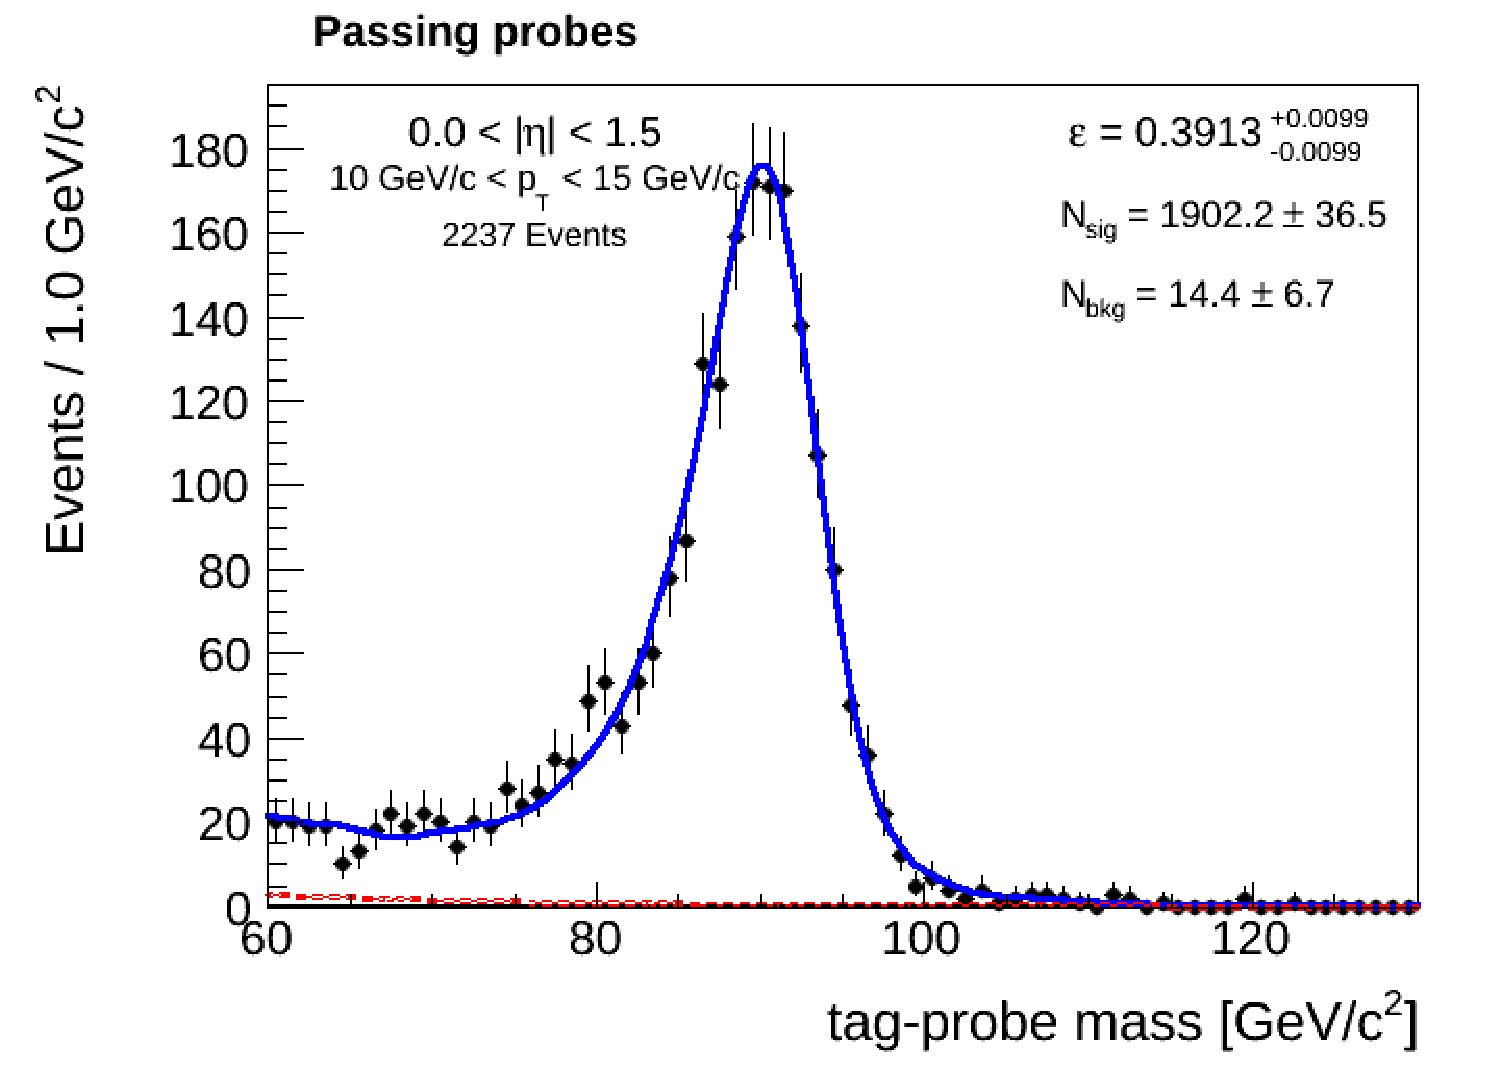
\includegraphics[width=0.45\textwidth]{figures/ElectronSelectionEffMassFitPass_EtaPtBin0.pdf}
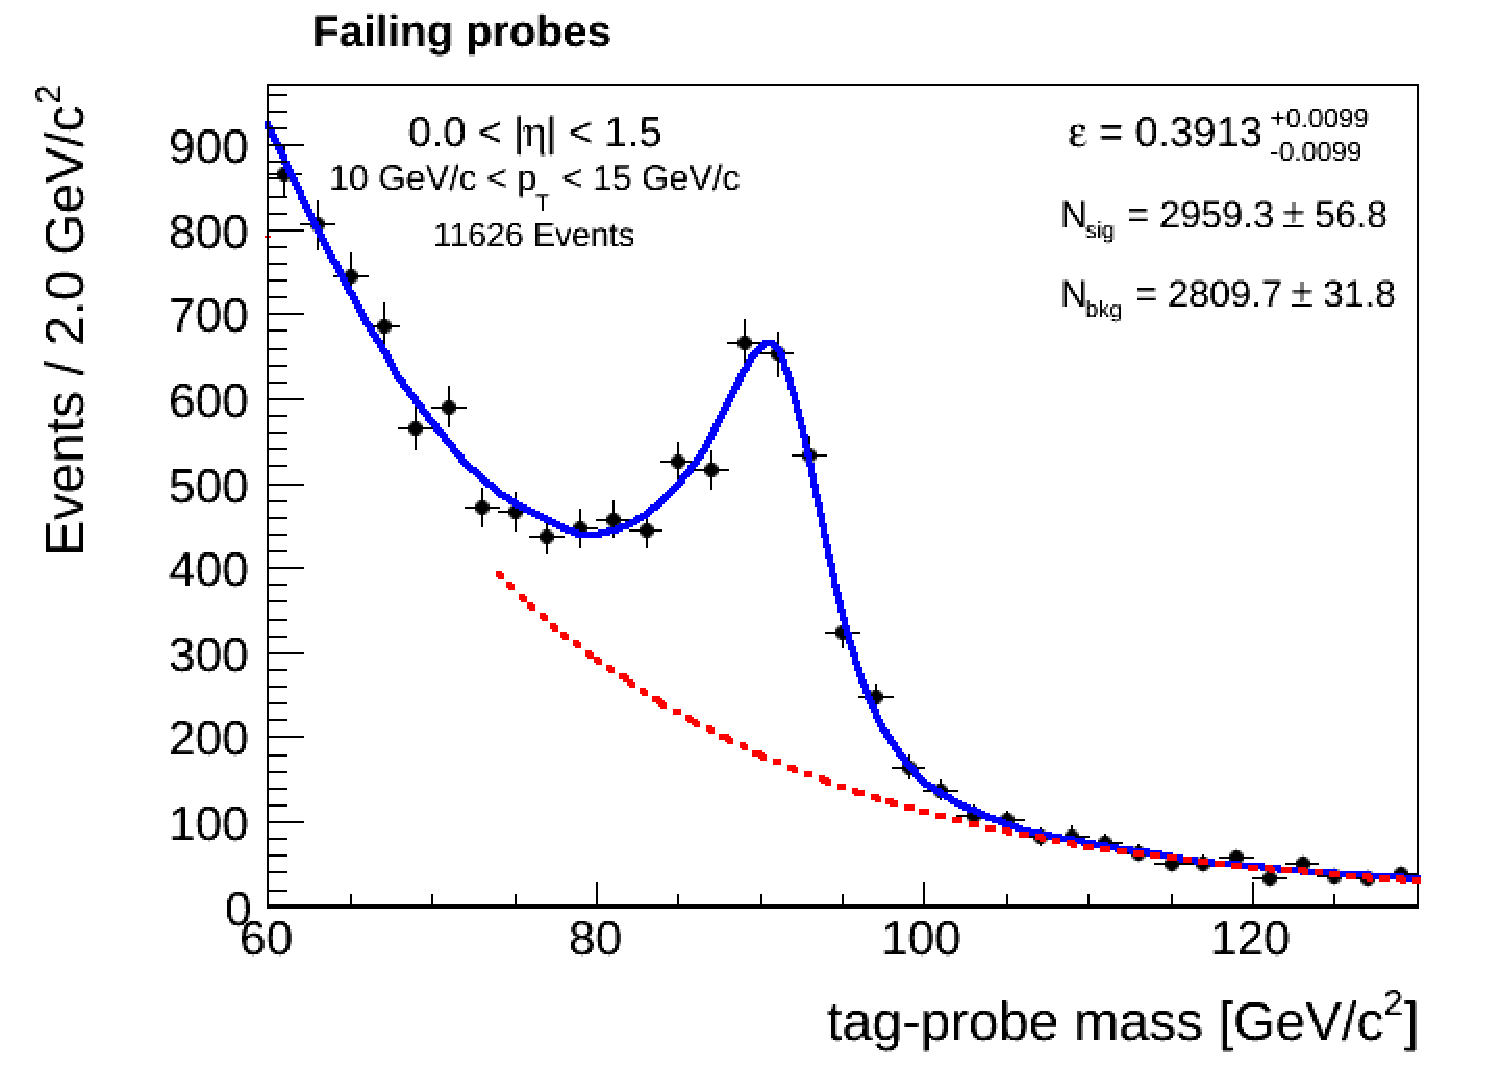
\includegraphics[width=0.45\textwidth]{figures/ElectronSelectionEffMassFitFail_EtaPtBin0.pdf}
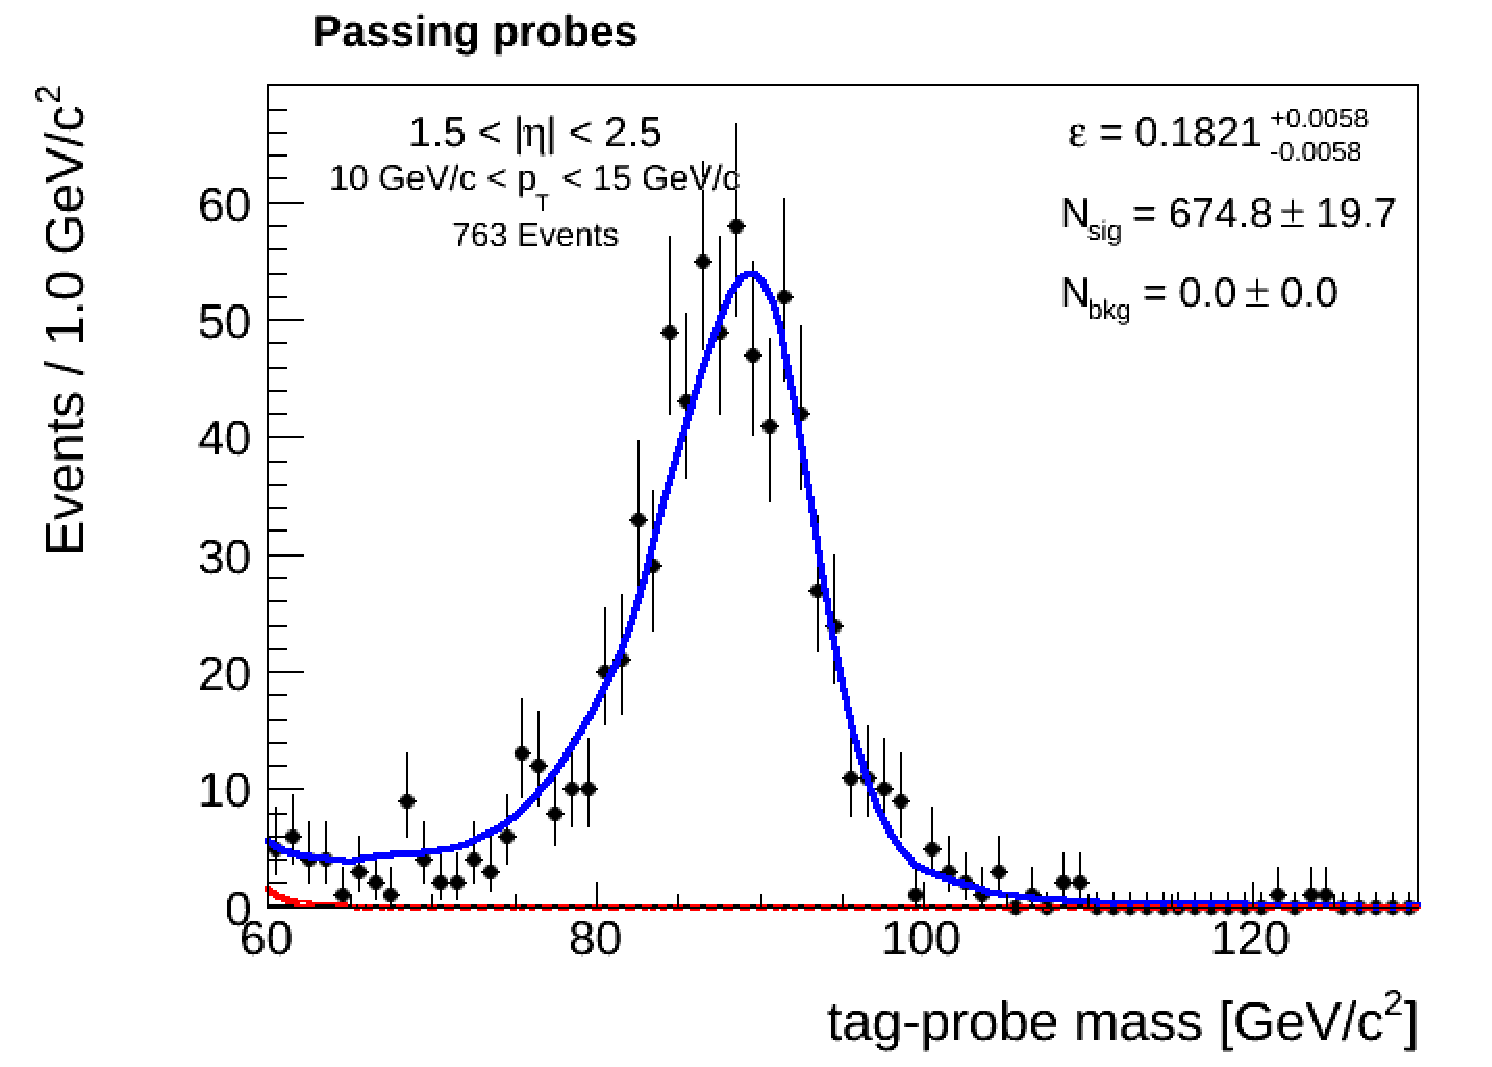
\includegraphics[width=0.45\textwidth]{figures/ElectronSelectionEffMassFitPass_EtaPtBin1.pdf}
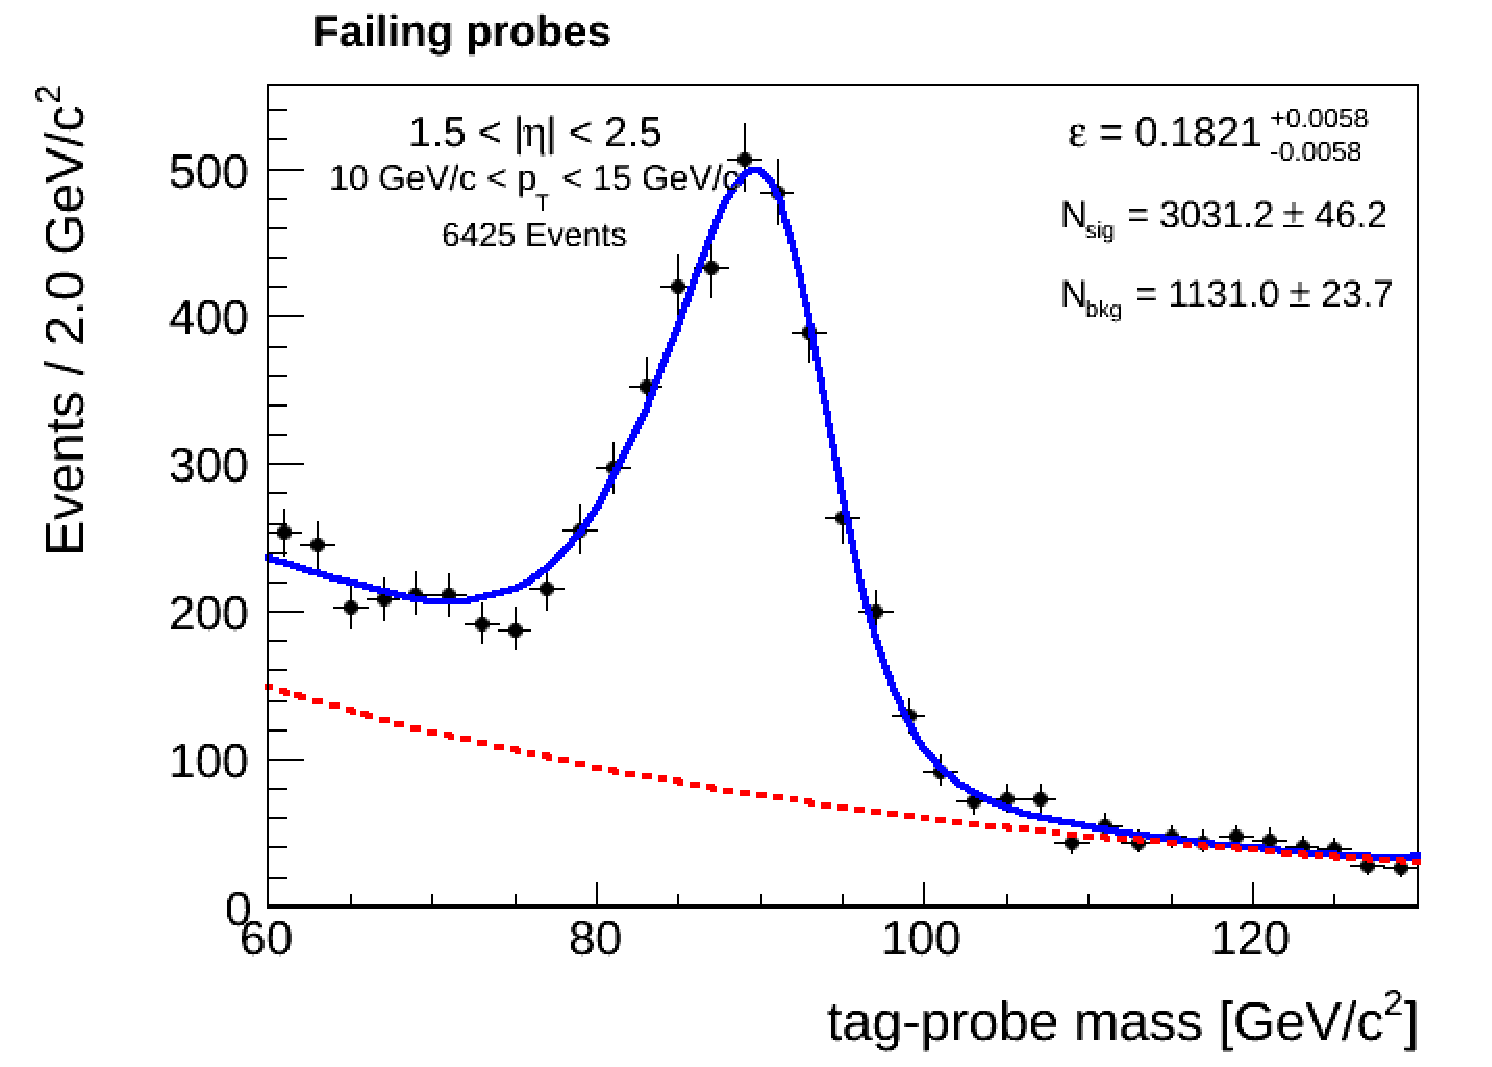
\includegraphics[width=0.45\textwidth]{figures/ElectronSelectionEffMassFitFail_EtaPtBin1.pdf}
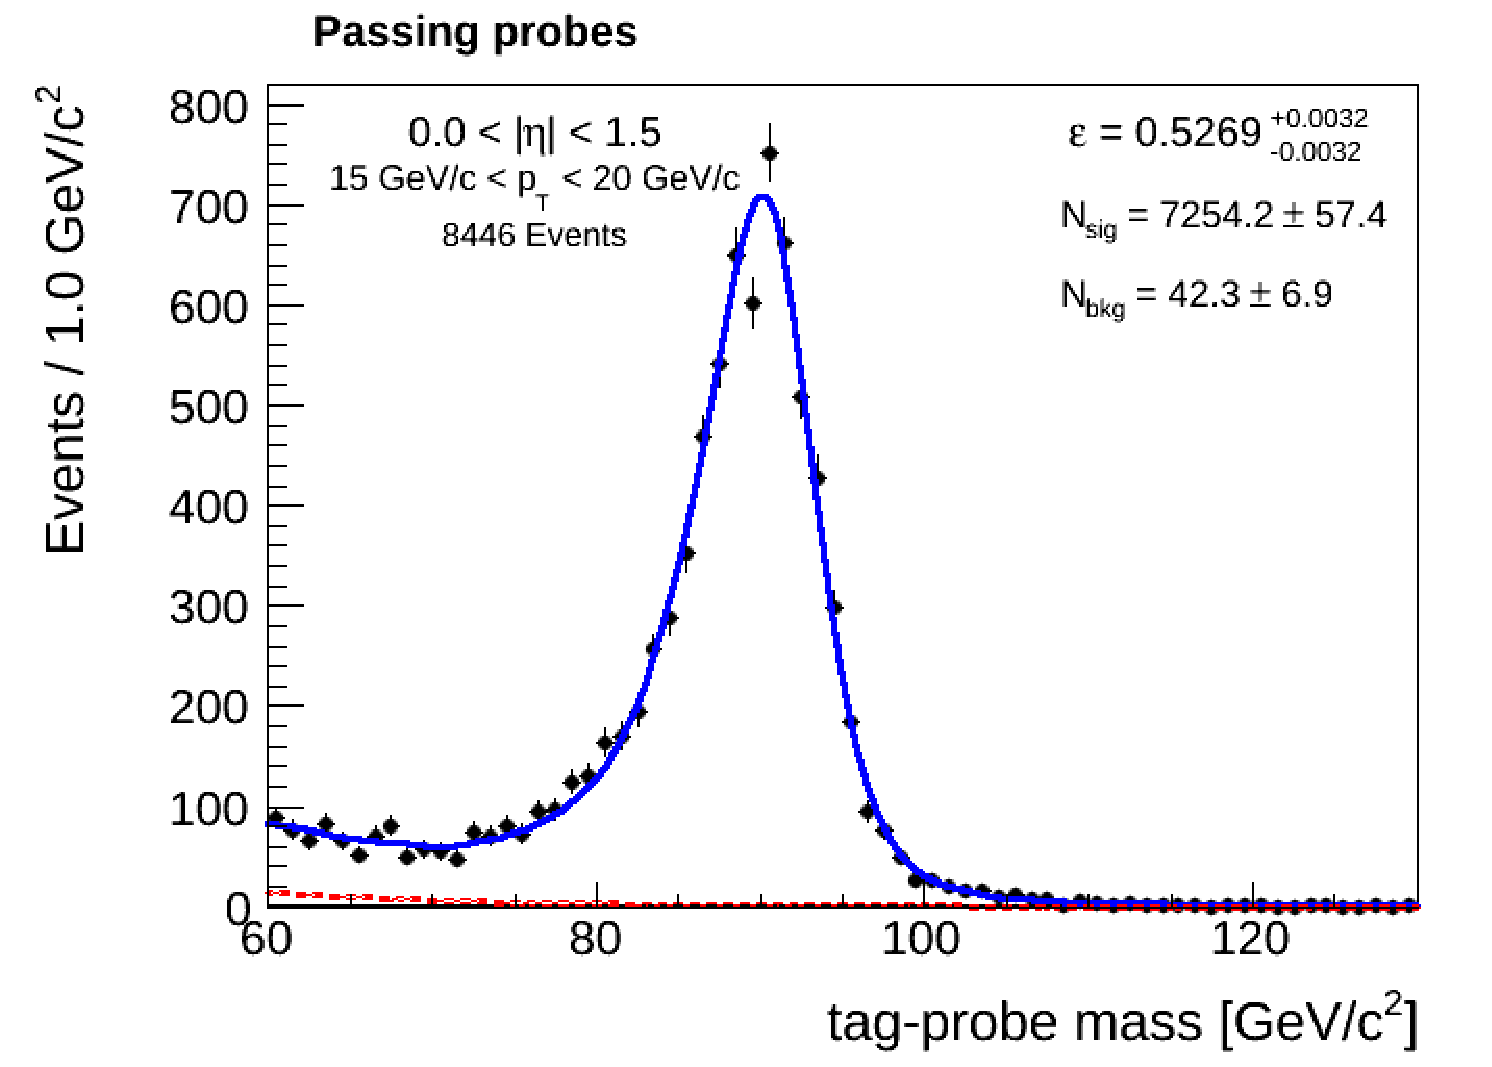
\includegraphics[width=0.45\textwidth]{figures/ElectronSelectionEffMassFitPass_EtaPtBin2.pdf}
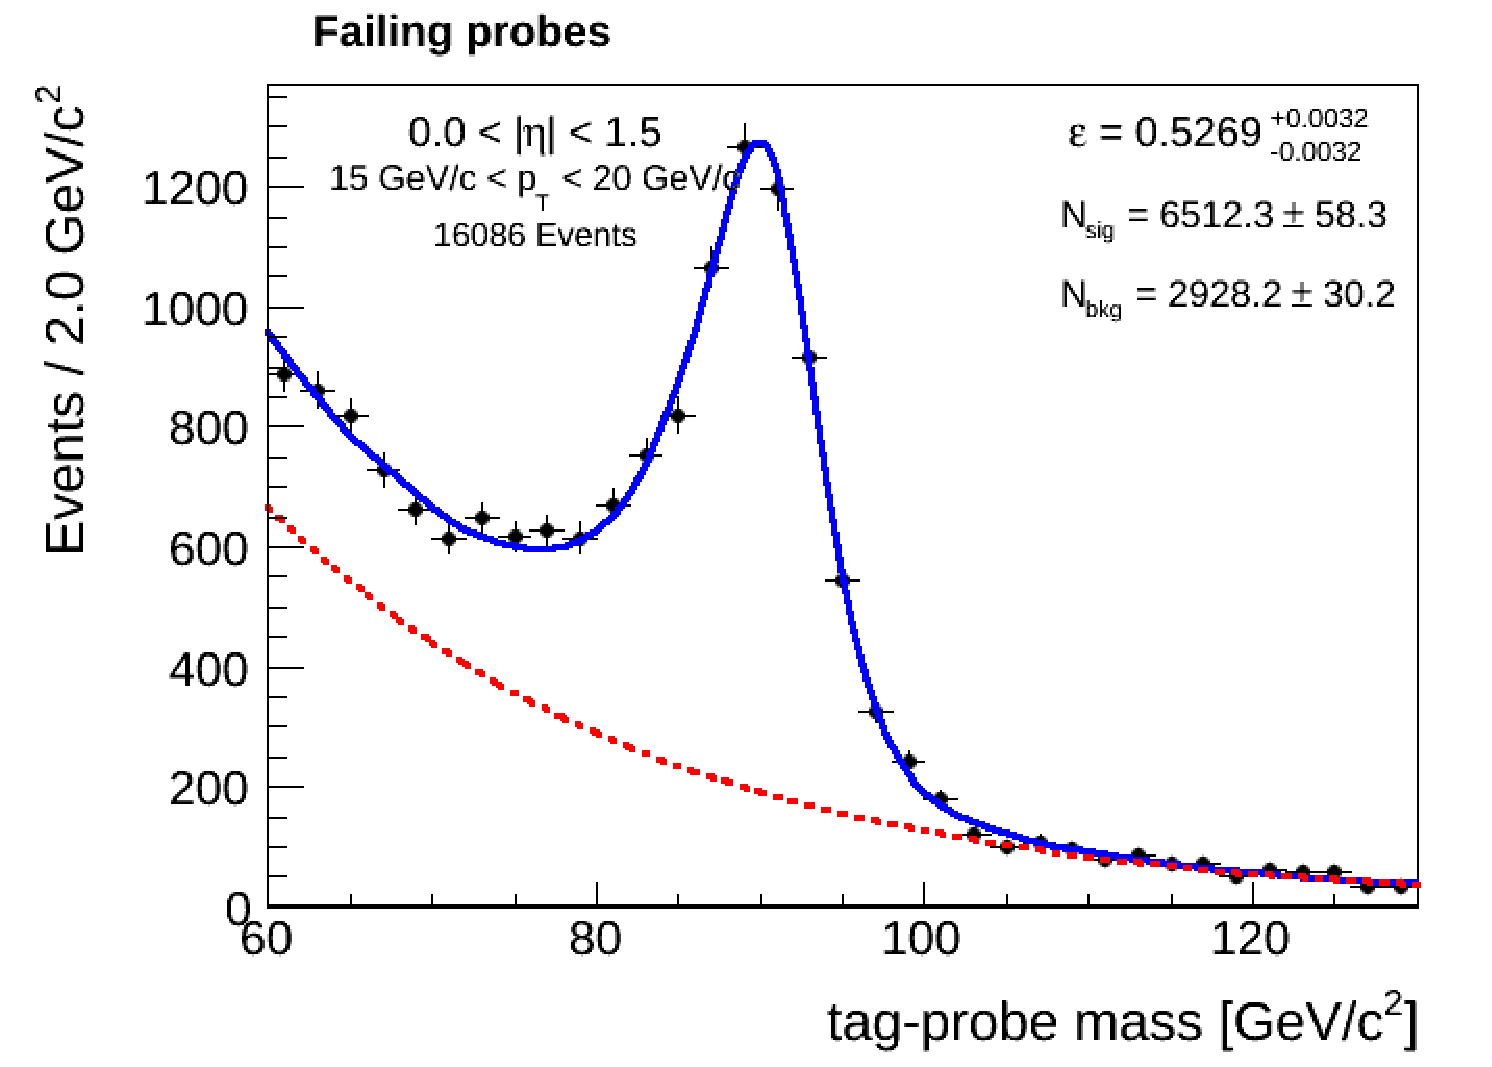
\includegraphics[width=0.45\textwidth]{figures/ElectronSelectionEffMassFitFail_EtaPtBin2.pdf}
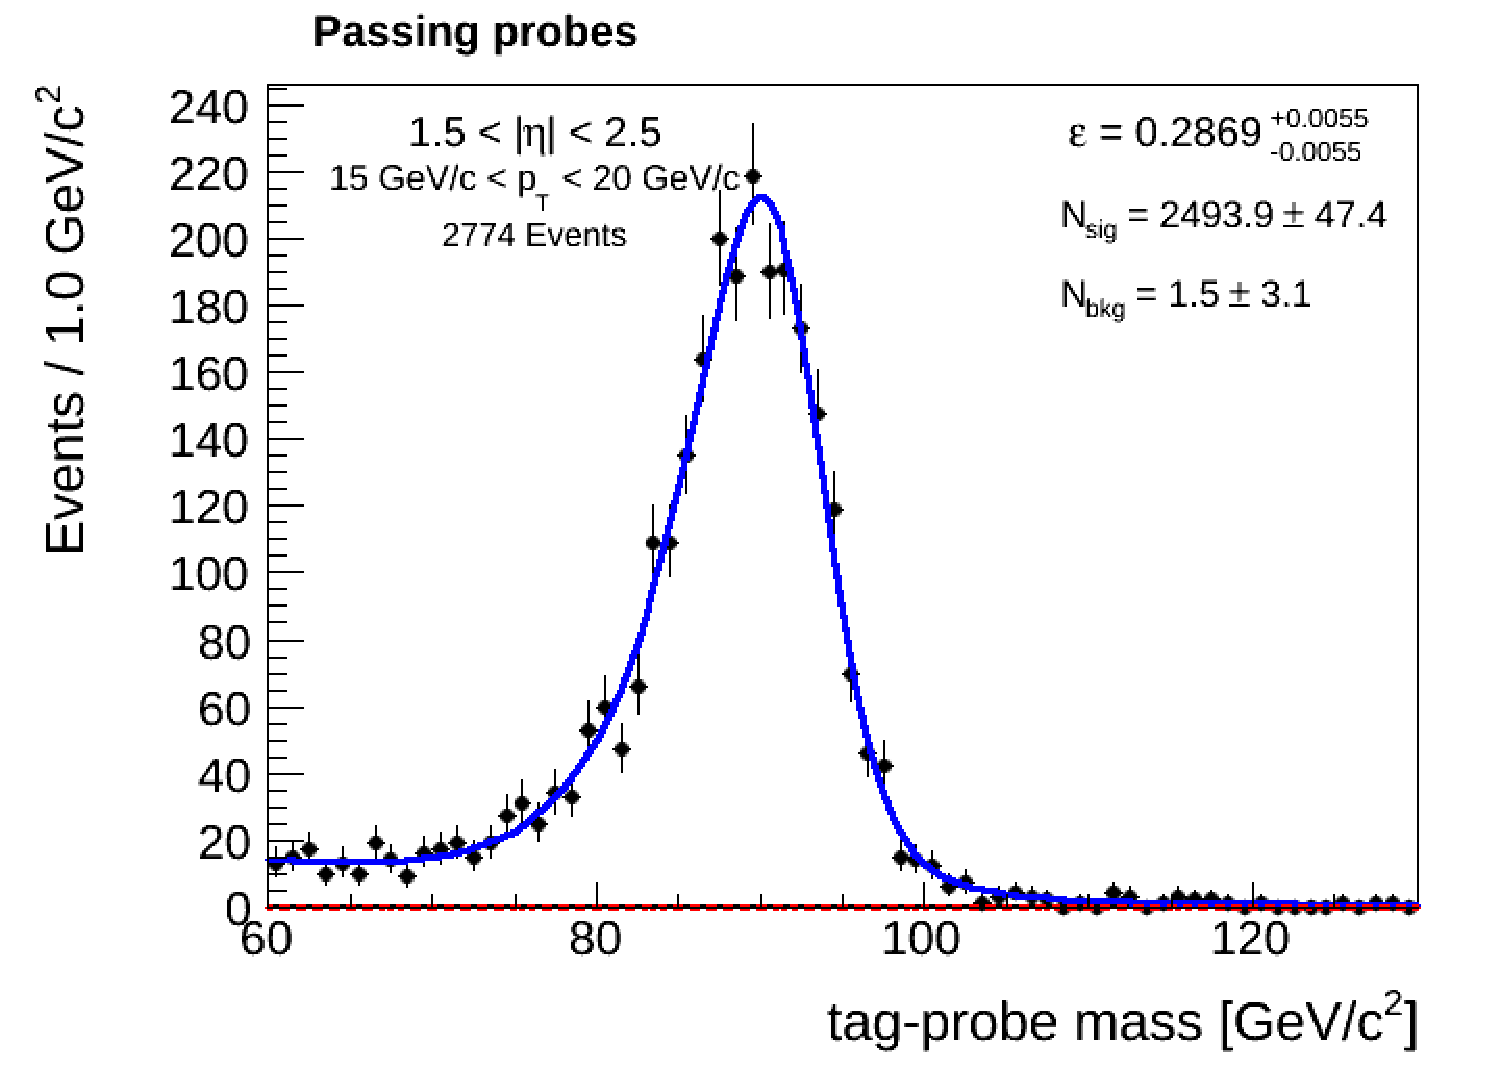
\includegraphics[width=0.45\textwidth]{figures/ElectronSelectionEffMassFitPass_EtaPtBin3.pdf}
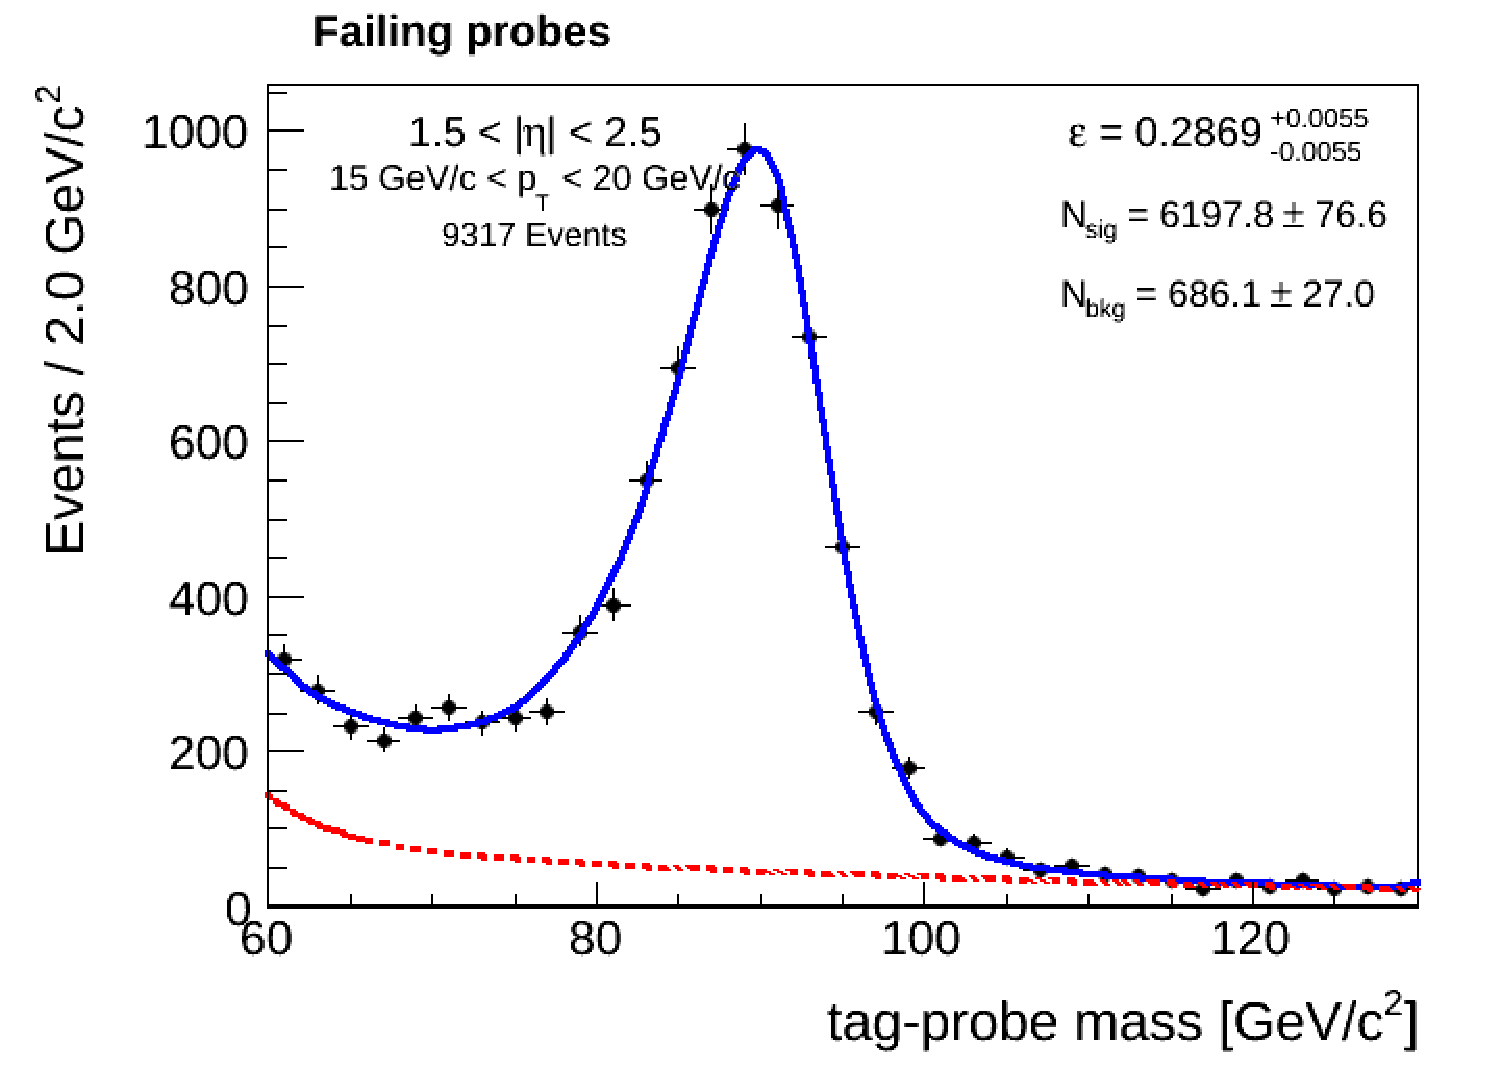
\includegraphics[width=0.45\textwidth]{figures/ElectronSelectionEffMassFitFail_EtaPtBin3.pdf}
\caption{Dielectron mass fits for the selection efficiency measurement for electrons with
$p_{T}$ less than $20$\GeV.}
\label{fig:ele_selectionEfficiency_massfits_lowPt}
\end{center}
\end{figure}

\newpage 

\begin{figure}[!htbp]
\begin{center}
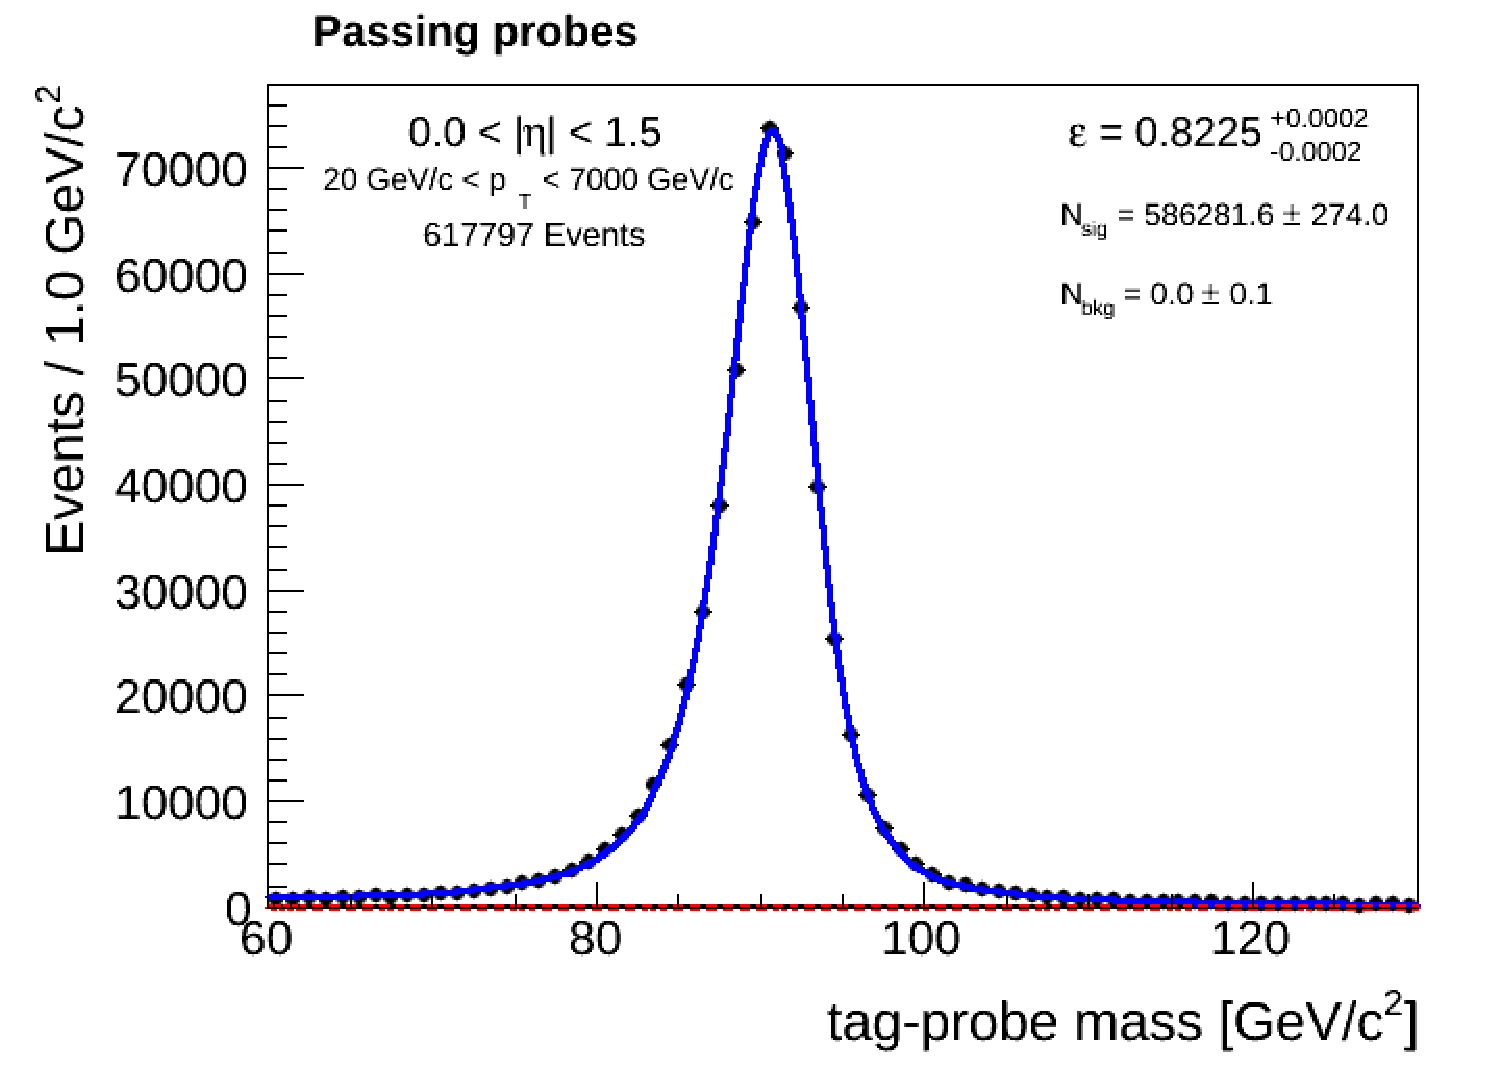
\includegraphics[width=0.45\textwidth]{figures/ElectronSelectionEffMassFitPass_EtaPtBin4.pdf}
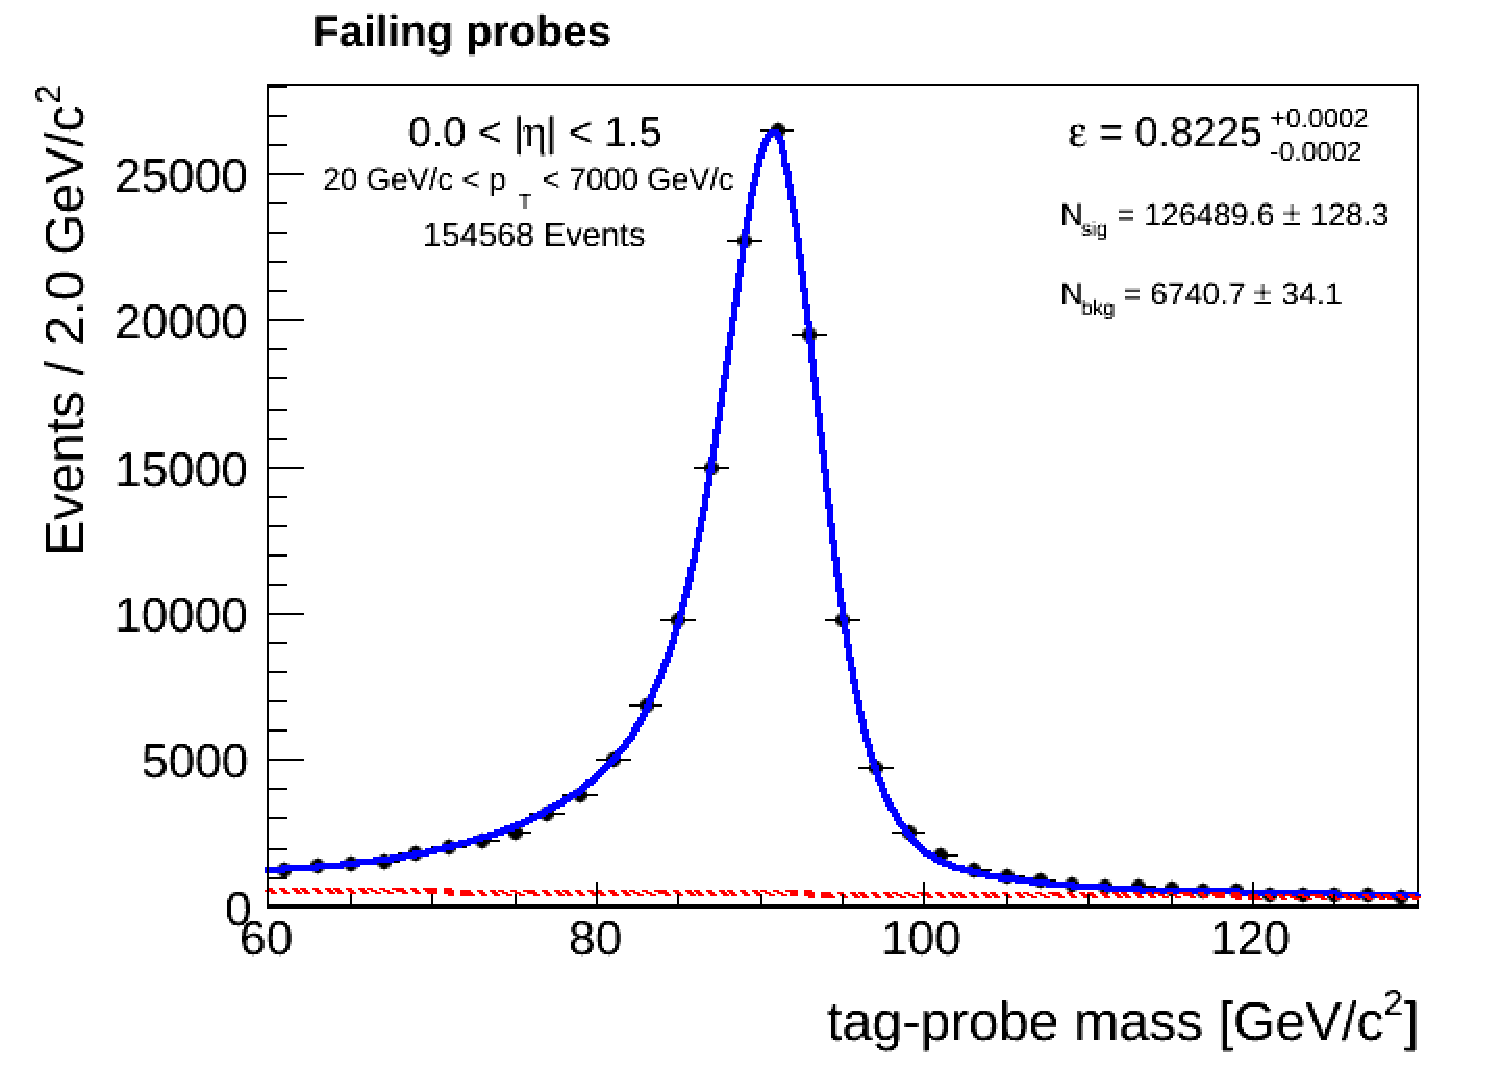
\includegraphics[width=0.45\textwidth]{figures/ElectronSelectionEffMassFitFail_EtaPtBin4.pdf}
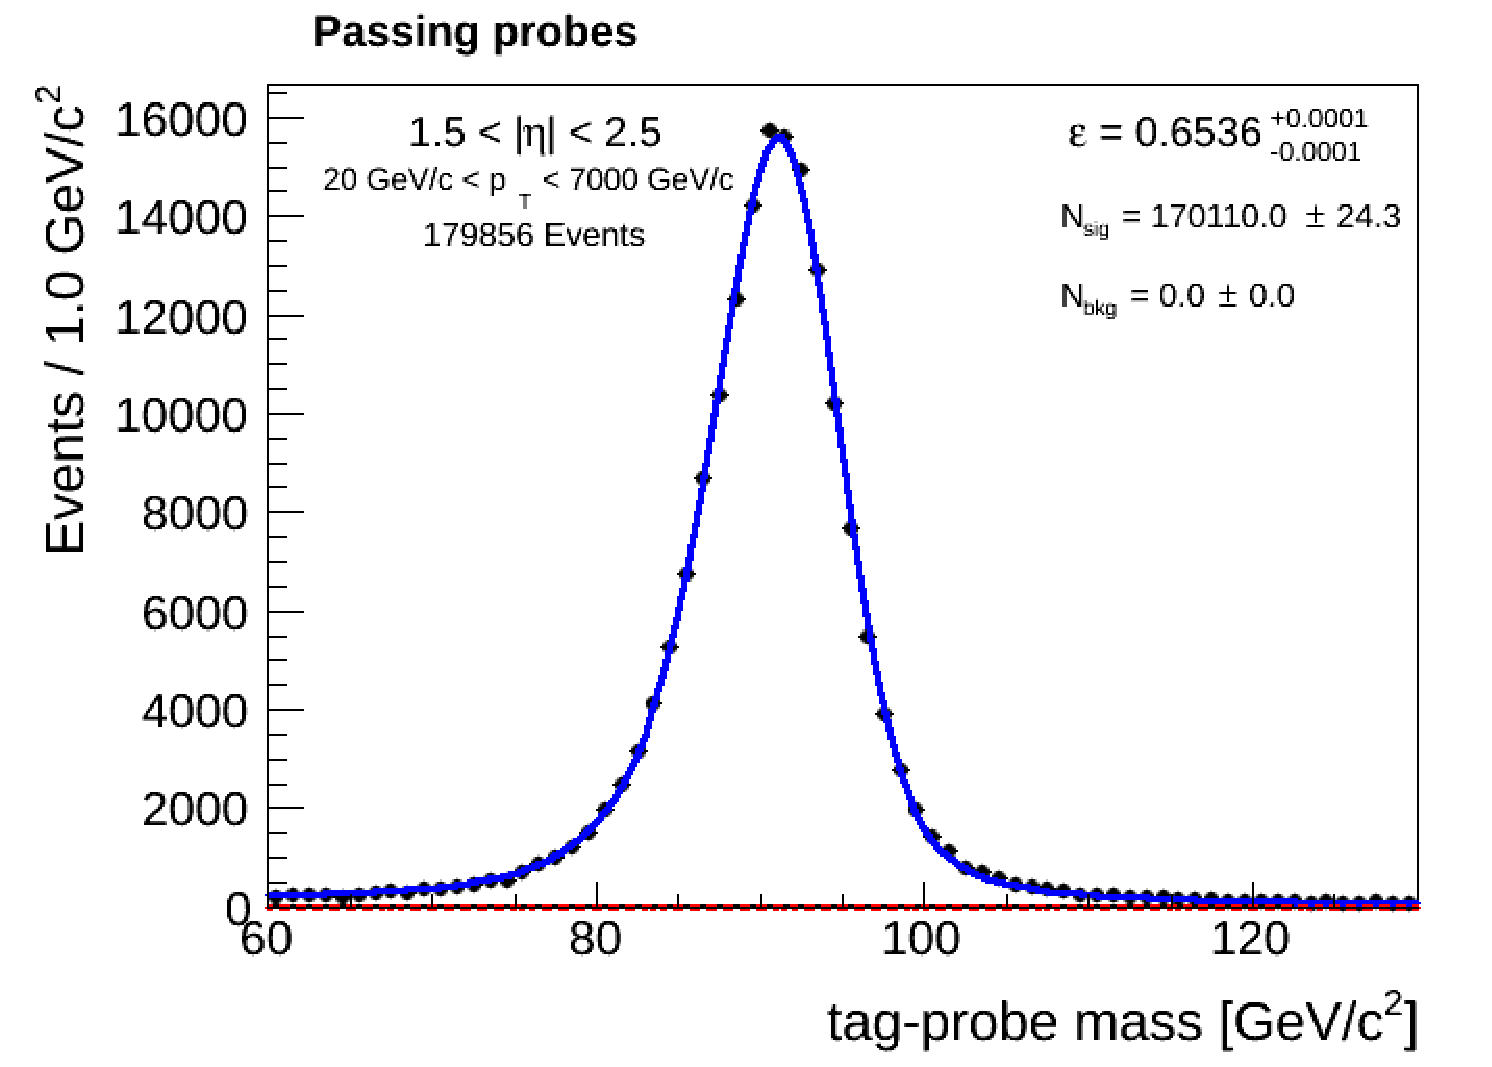
\includegraphics[width=0.45\textwidth]{figures/ElectronSelectionEffMassFitPass_EtaPtBin5.pdf}
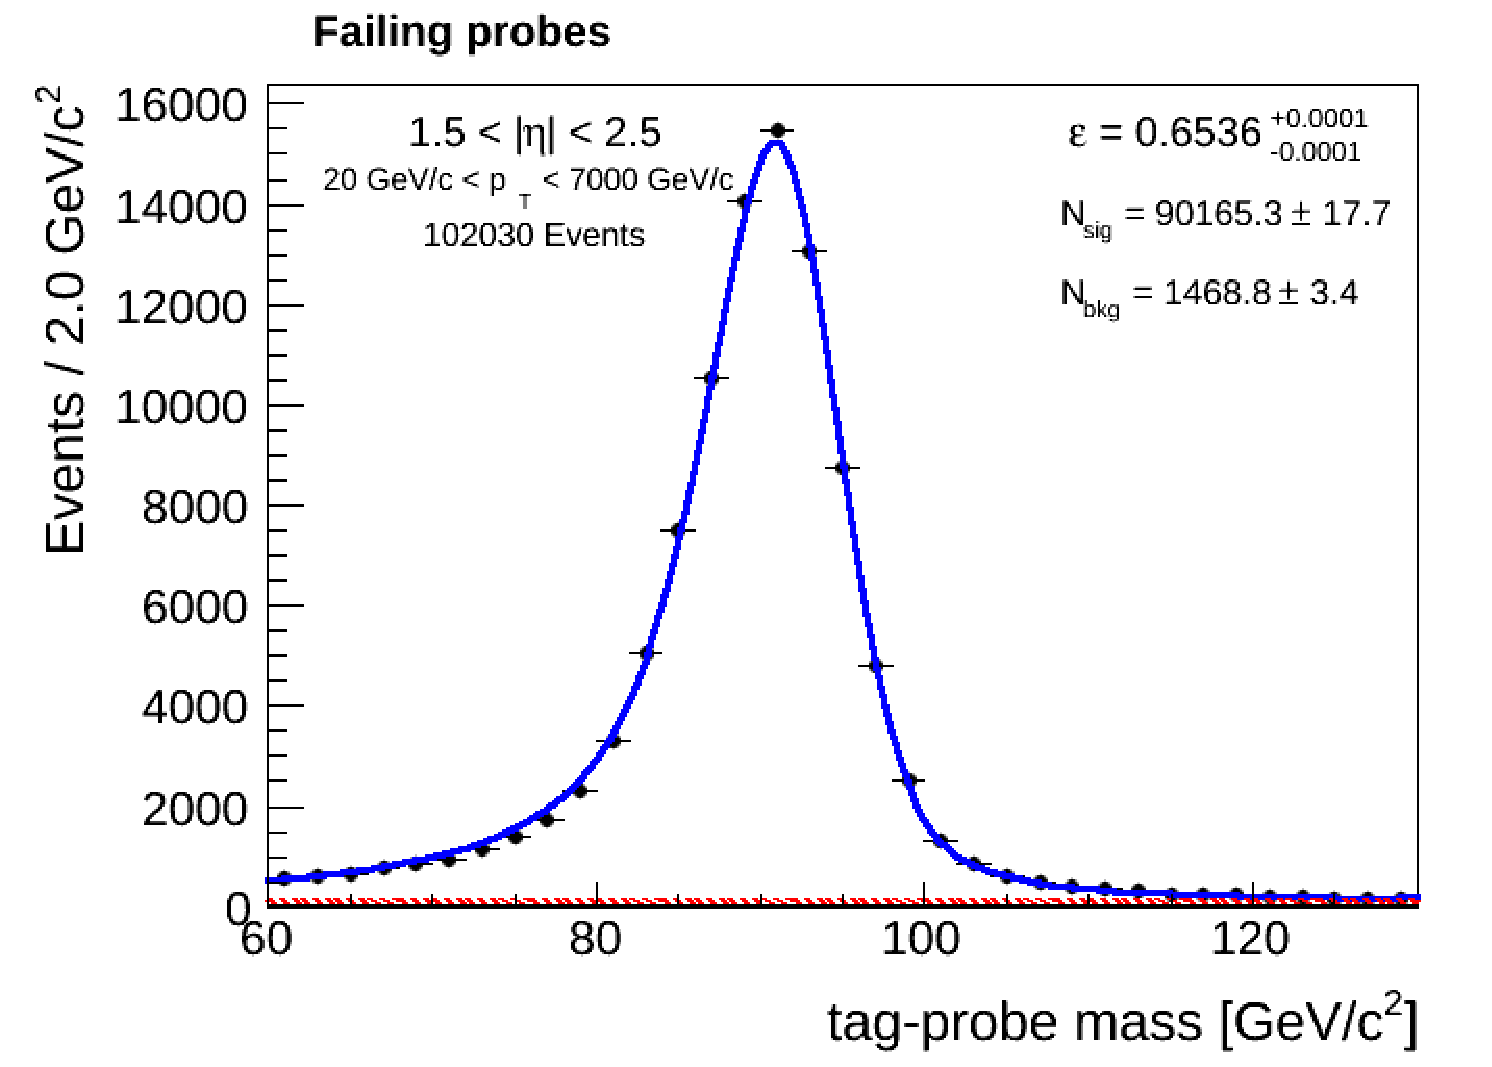
\includegraphics[width=0.45\textwidth]{figures/ElectronSelectionEffMassFitFail_EtaPtBin5.pdf}
\caption{Dielectron mass fits for the selection efficiency measurement for electrons with
$p_{T}$ greater than $20$\GeV.}
\label{fig:ele_selectionEfficiency_massfits_highPt}
\end{center}
\end{figure}


The electron selection efficiency is plotted as a function of the $p_{T}$ of the electron in Figure 
\ref{fig:ele_selectionEfficiency_VsPt} and as a function of the pseudorapidity of the electron
in Figure \ref{} for low $p_{T}$ and high $p_{T}$ electrons separately. Finally in Figures
\ref{fig:ele_selectionEfficiency_LowPt_VsPileup} and \ref{fig:ele_selectionEfficiency_HighPt_VsPileup}
we show the dependence of the efficiency on the amount of pileup, characterized by the
number of primary vertices reconstructed in the event and the pileup energy density 
in the event for low $p_{T}$ and high $p_{T}$ electrons respectively.

\begin{figure}[!htbp]
\begin{center}
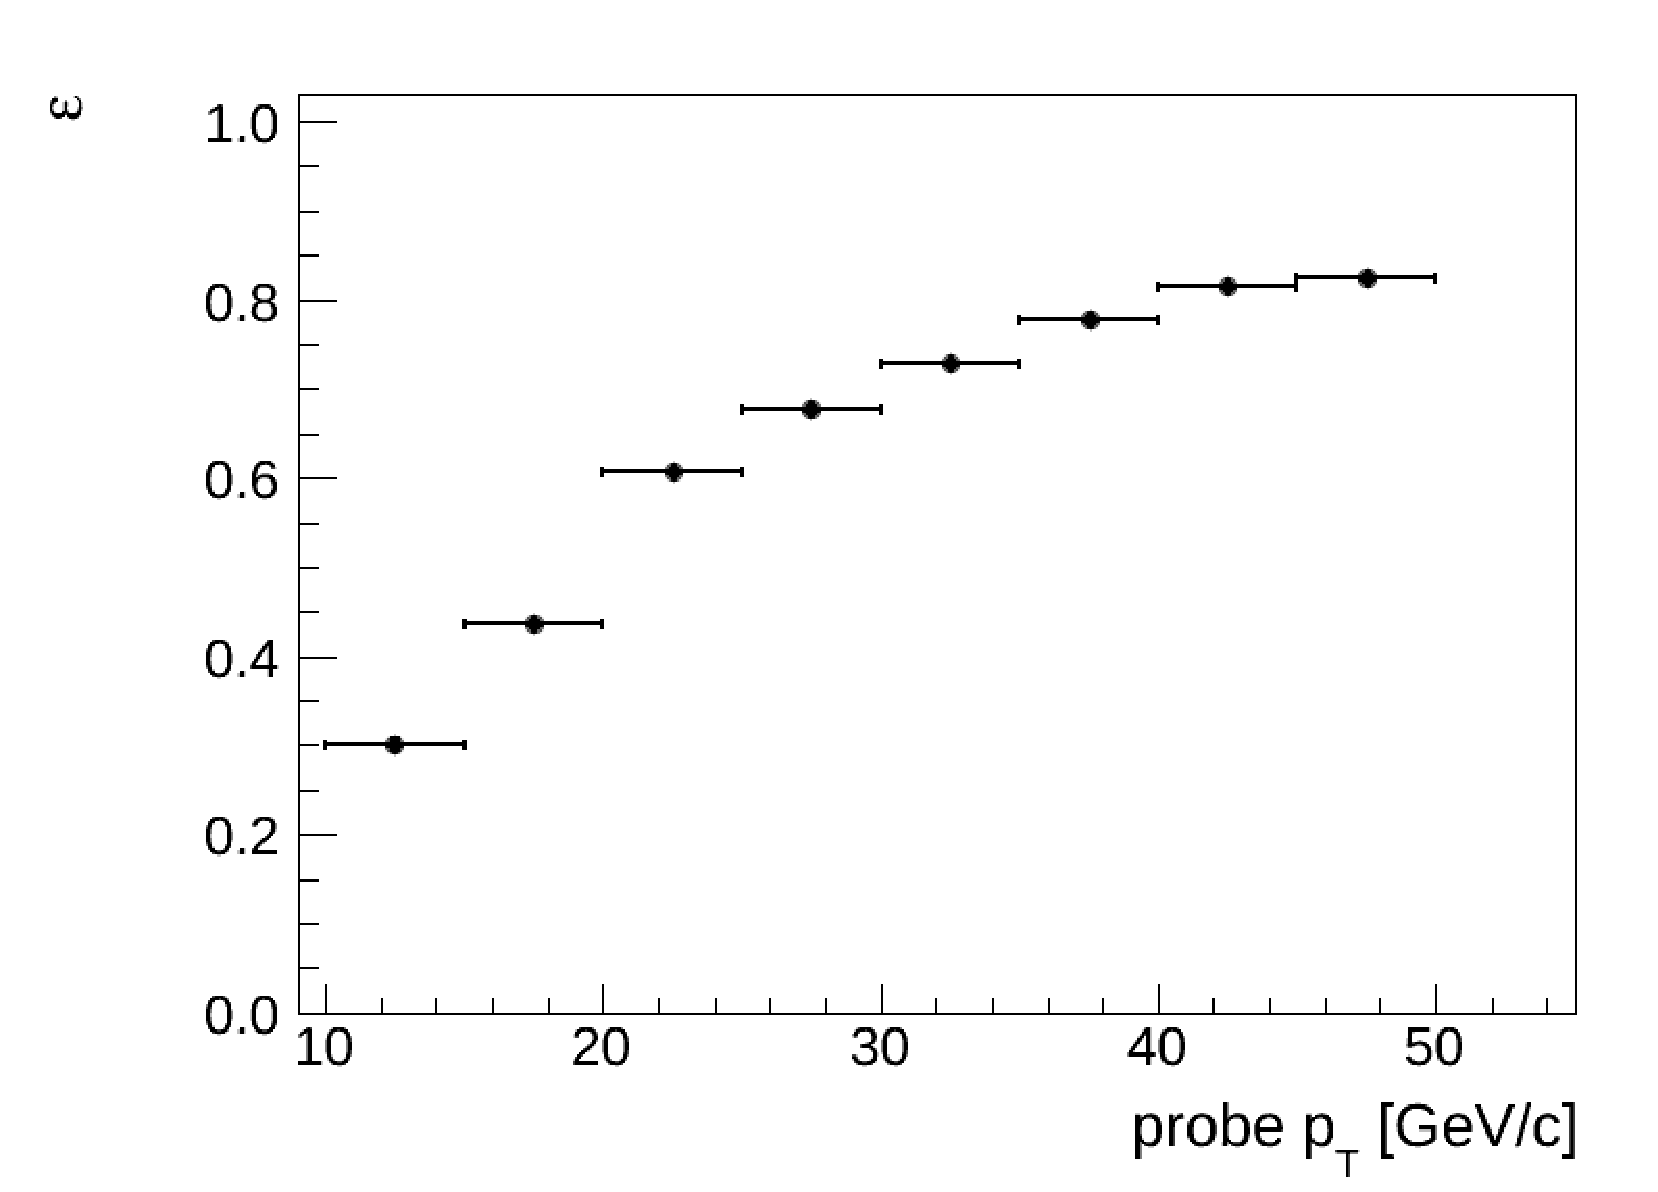
\includegraphics[width=0.45\textwidth]{figures/ElectronEff_VsPt.pdf}
\caption{Electron selection efficiency as a function of the $p_{T}$ of the electron.}
\label{fig:ele_selectionEfficiency_VsPt}
\end{center}
\end{figure}


\begin{figure}[!htbp]
\begin{center}
\subfigure[$10$ \GeV\ $ < p_{T} \le 20$ \GeV]{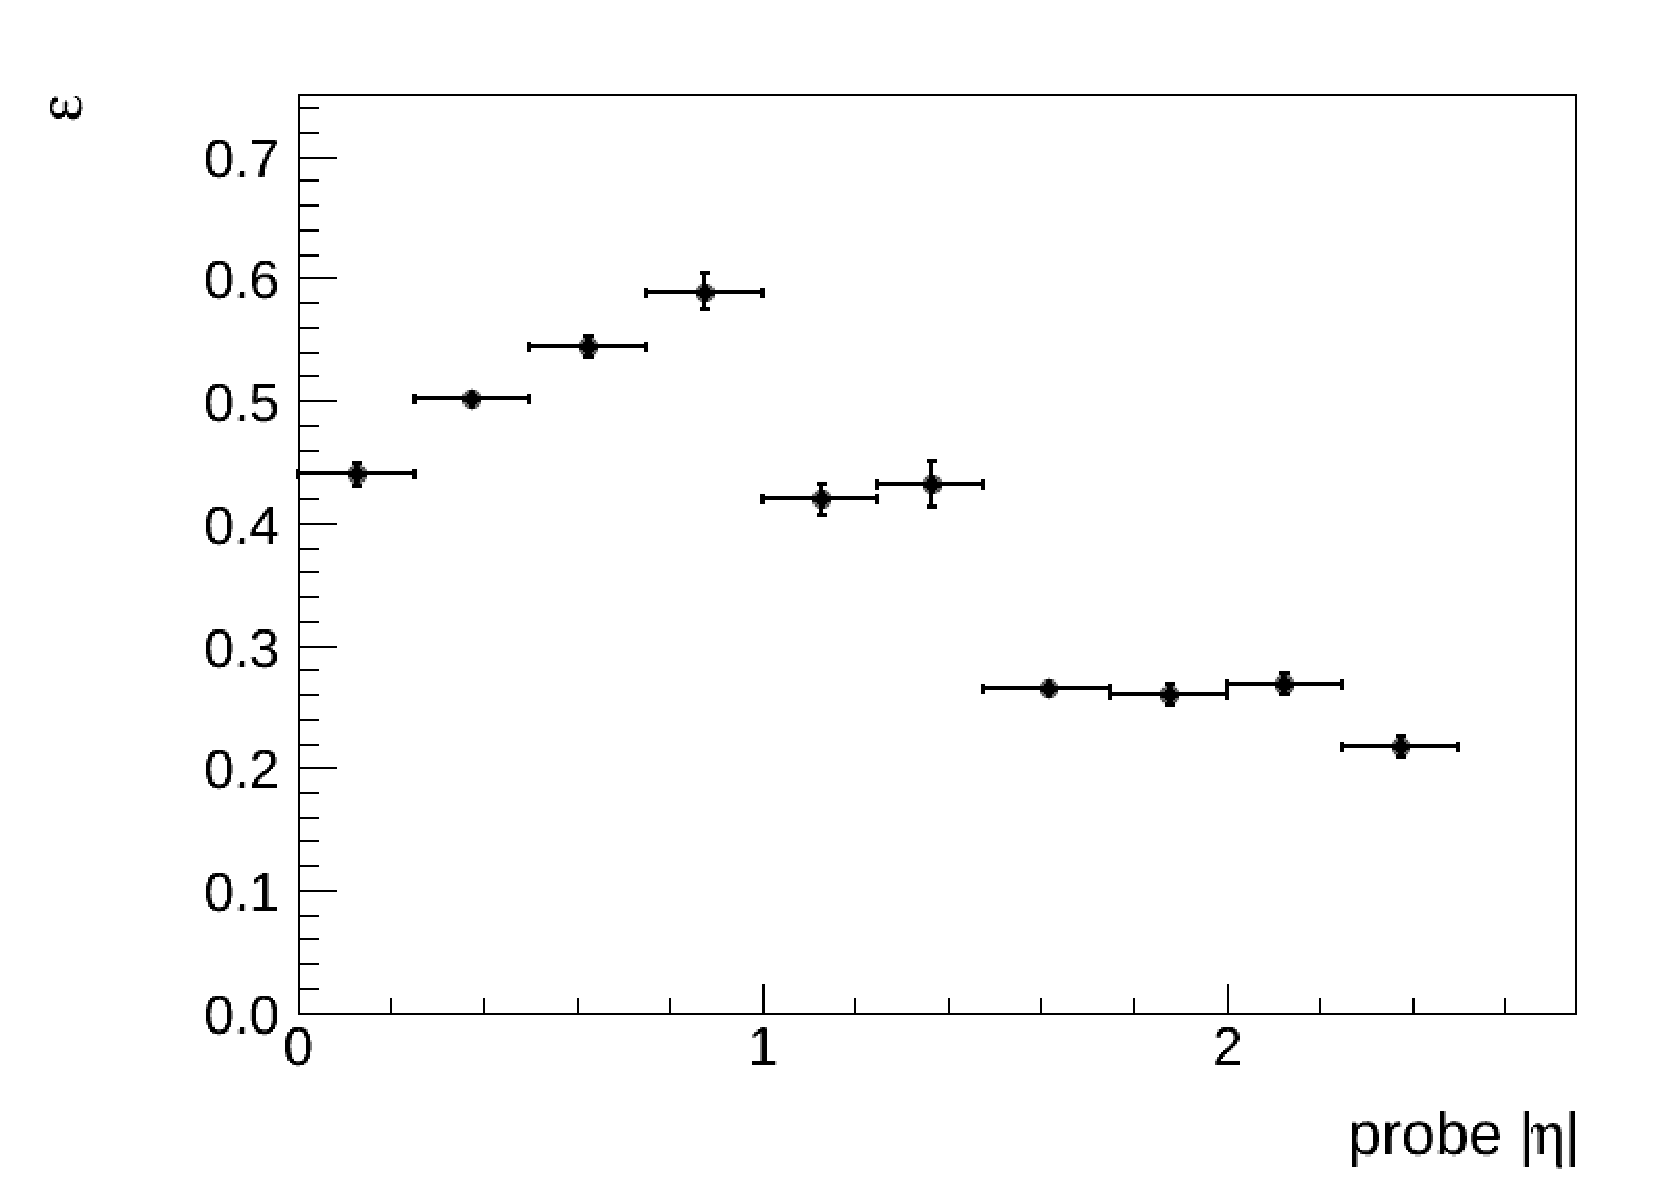
\includegraphics[width=0.45\textwidth]{figures/ElectronEff_LowPt_VsEta.pdf}}
\subfigure[$p_{T} > 20$]{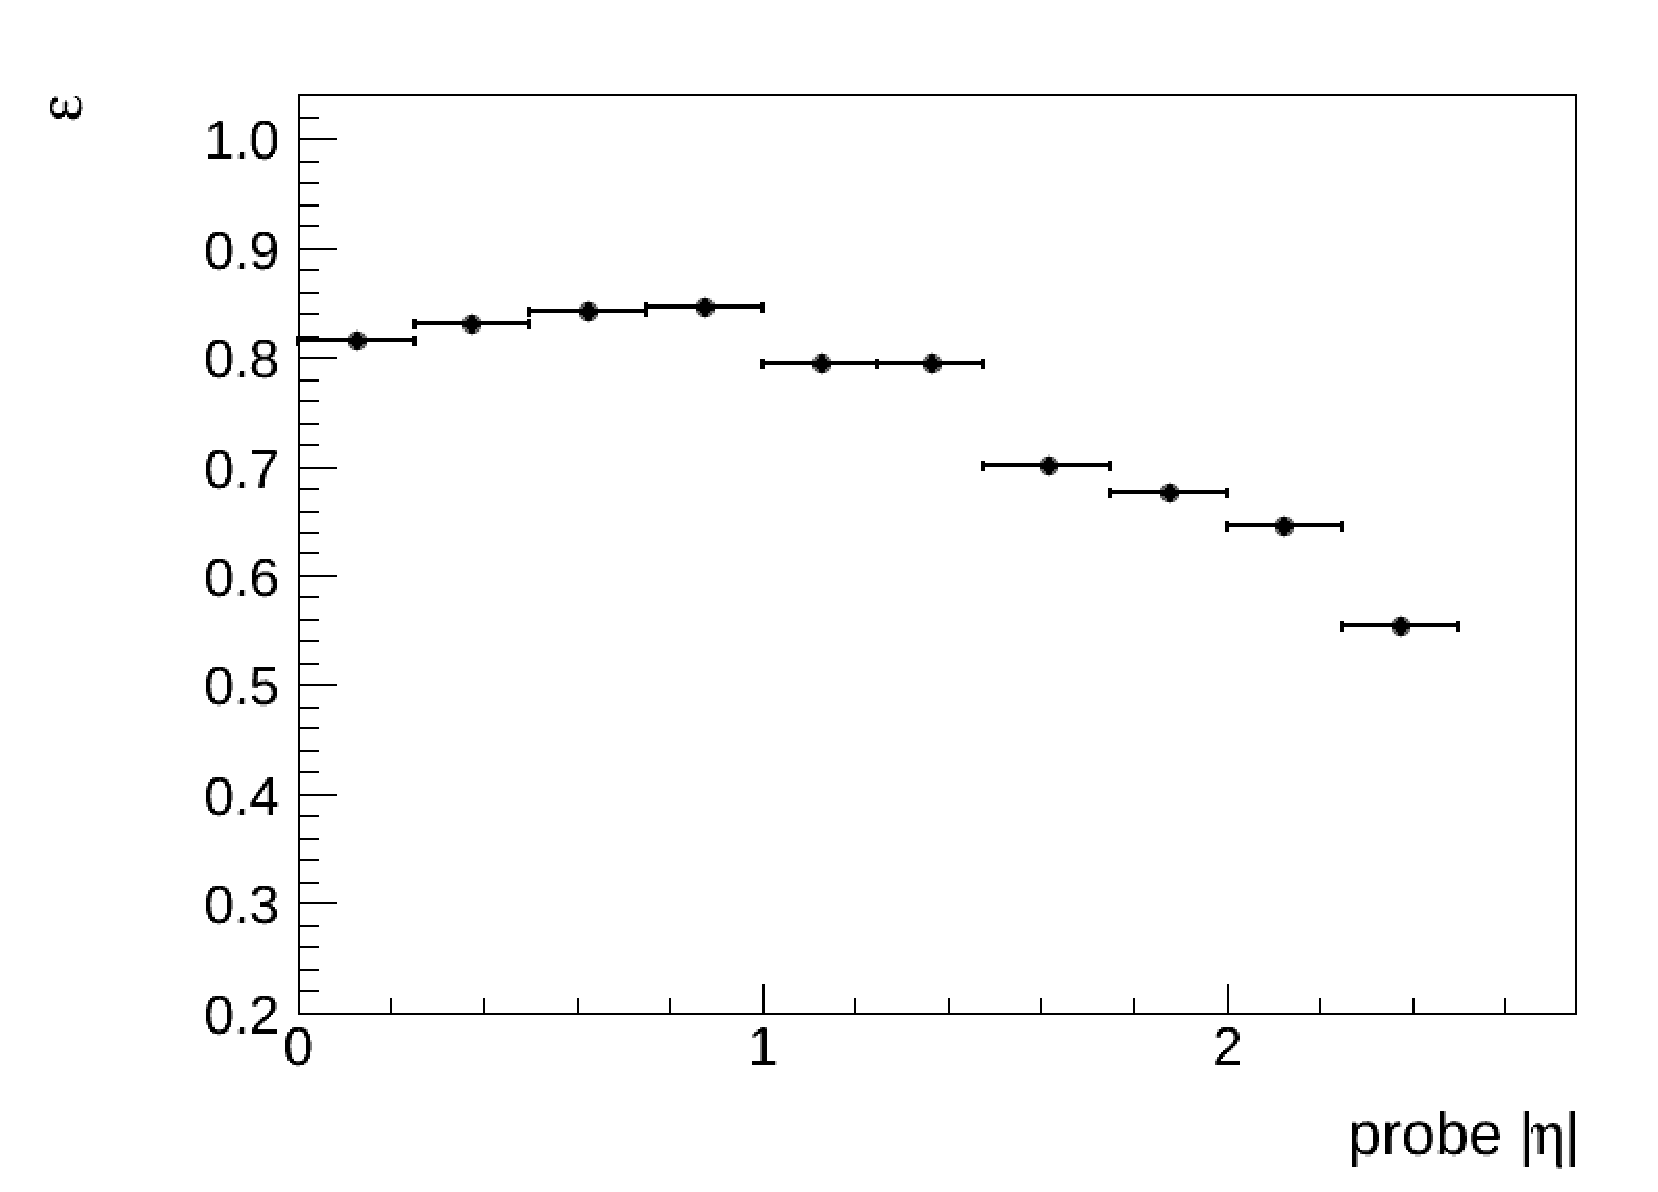
\includegraphics[width=0.45\textwidth]{figures/ElectronEff_HighPt_VsEta.pdf}}
\caption{Electron selection efficiency as a function of the $p_{T}$ of the electron.}
\label{fig:ele_selectionEfficiency_VsEta}
\end{center}
\end{figure}



\begin{figure}[!htbp]
\begin{center}
\subfigure[Number of reconstructed primary vertices]{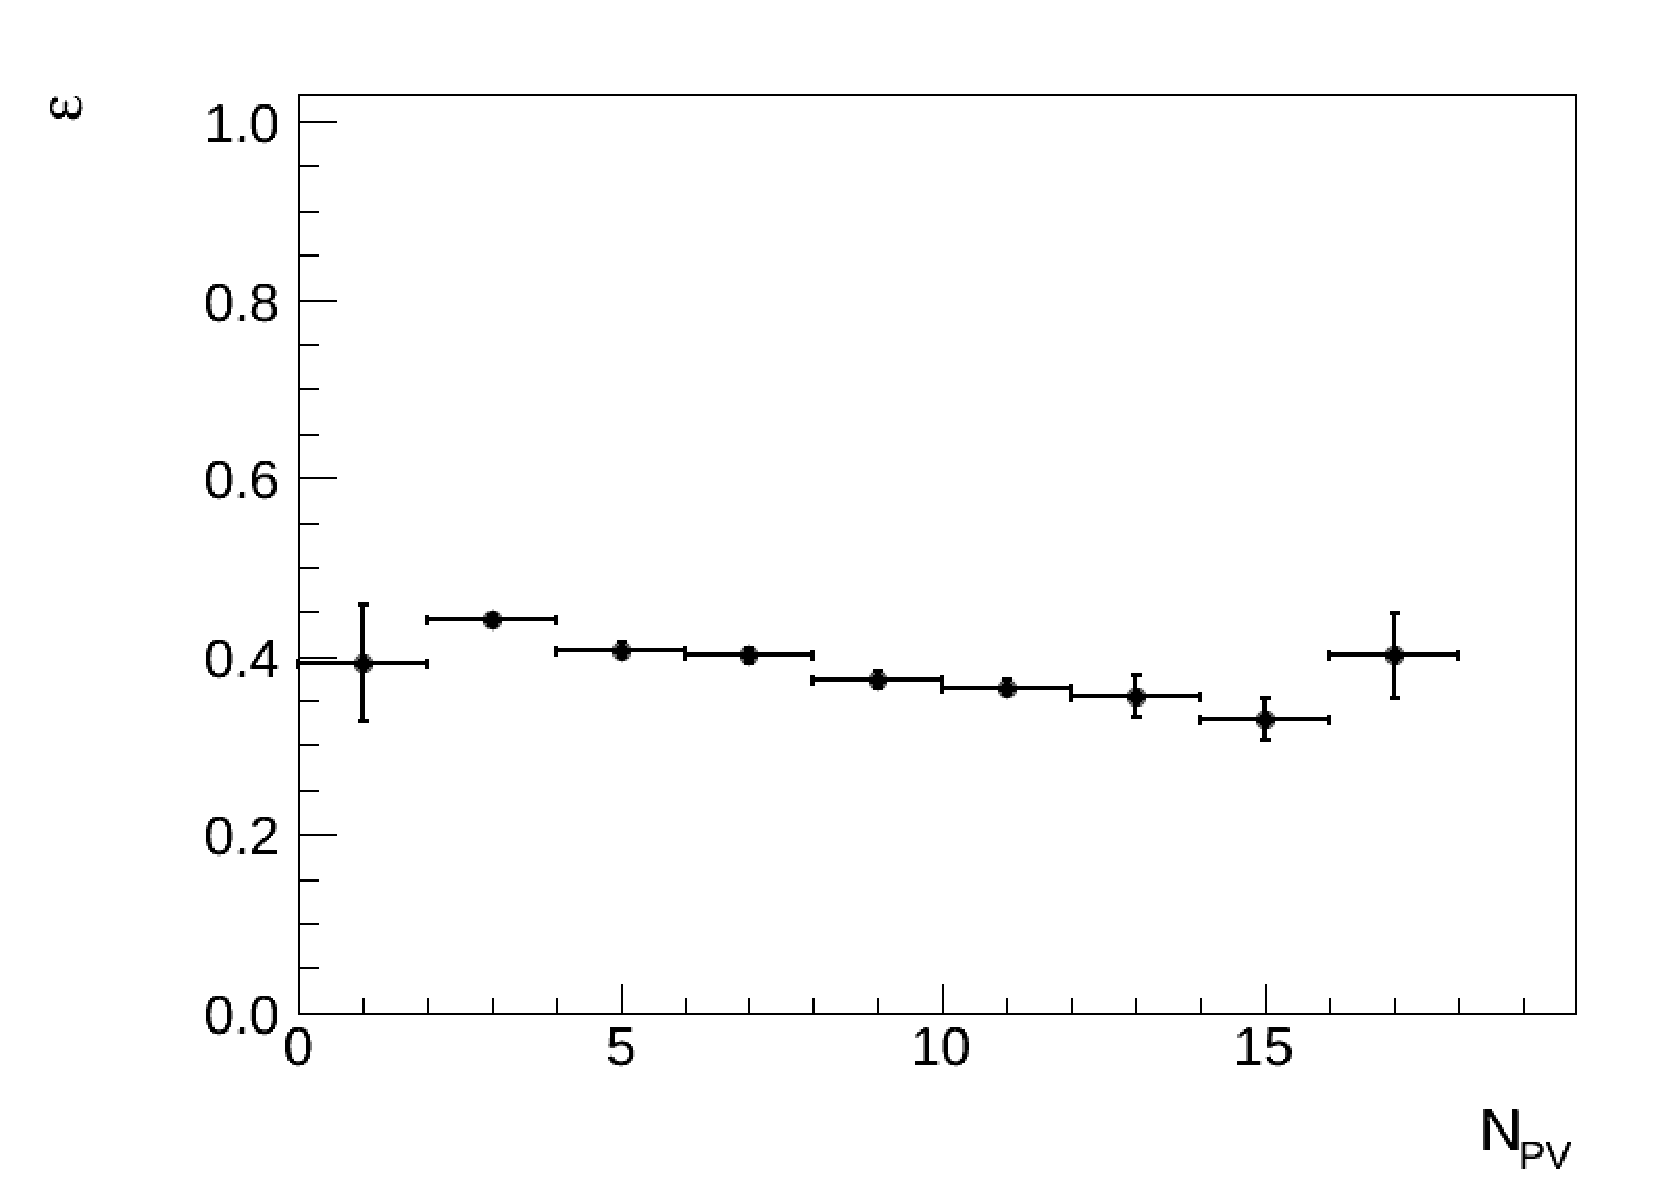
\includegraphics[width=0.45\textwidth]{figures/ElectronEff_LowPt_VsNVtx.pdf}}
\subfigure[Pileup energy density ($\rho$)]{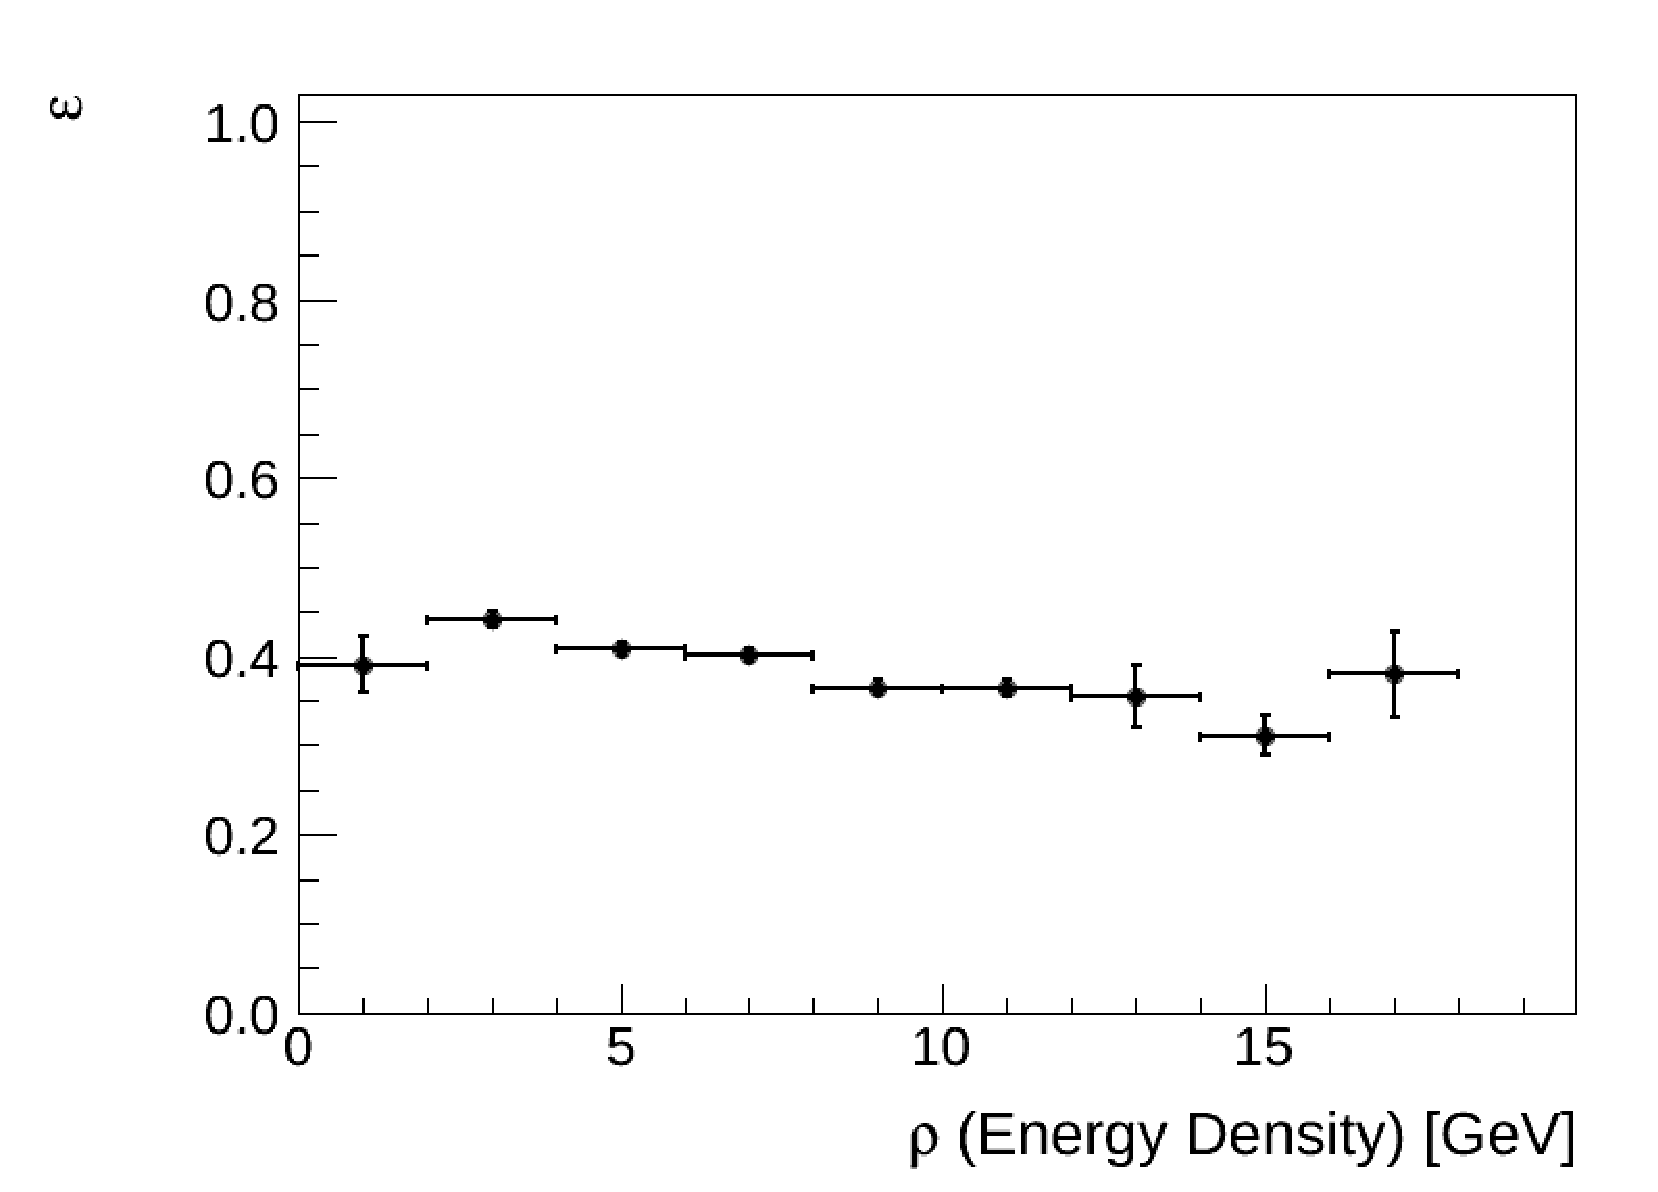
\includegraphics[width=0.45\textwidth]{figures/ElectronEff_LowPt_VsRho.pdf}}
\caption{Electron selection efficiency as a function of the number of reconstructed primary vertices
and the pileup energy density for electrons with $p_{T}$ between 10 and 20\GeV.}
\label{fig:ele_selectionEfficiency_LowPt_VsPileup}
\end{center}
\end{figure}



\begin{figure}[!htbp]
\begin{center}
\subfigure[Number of reconstructed primary vertices]{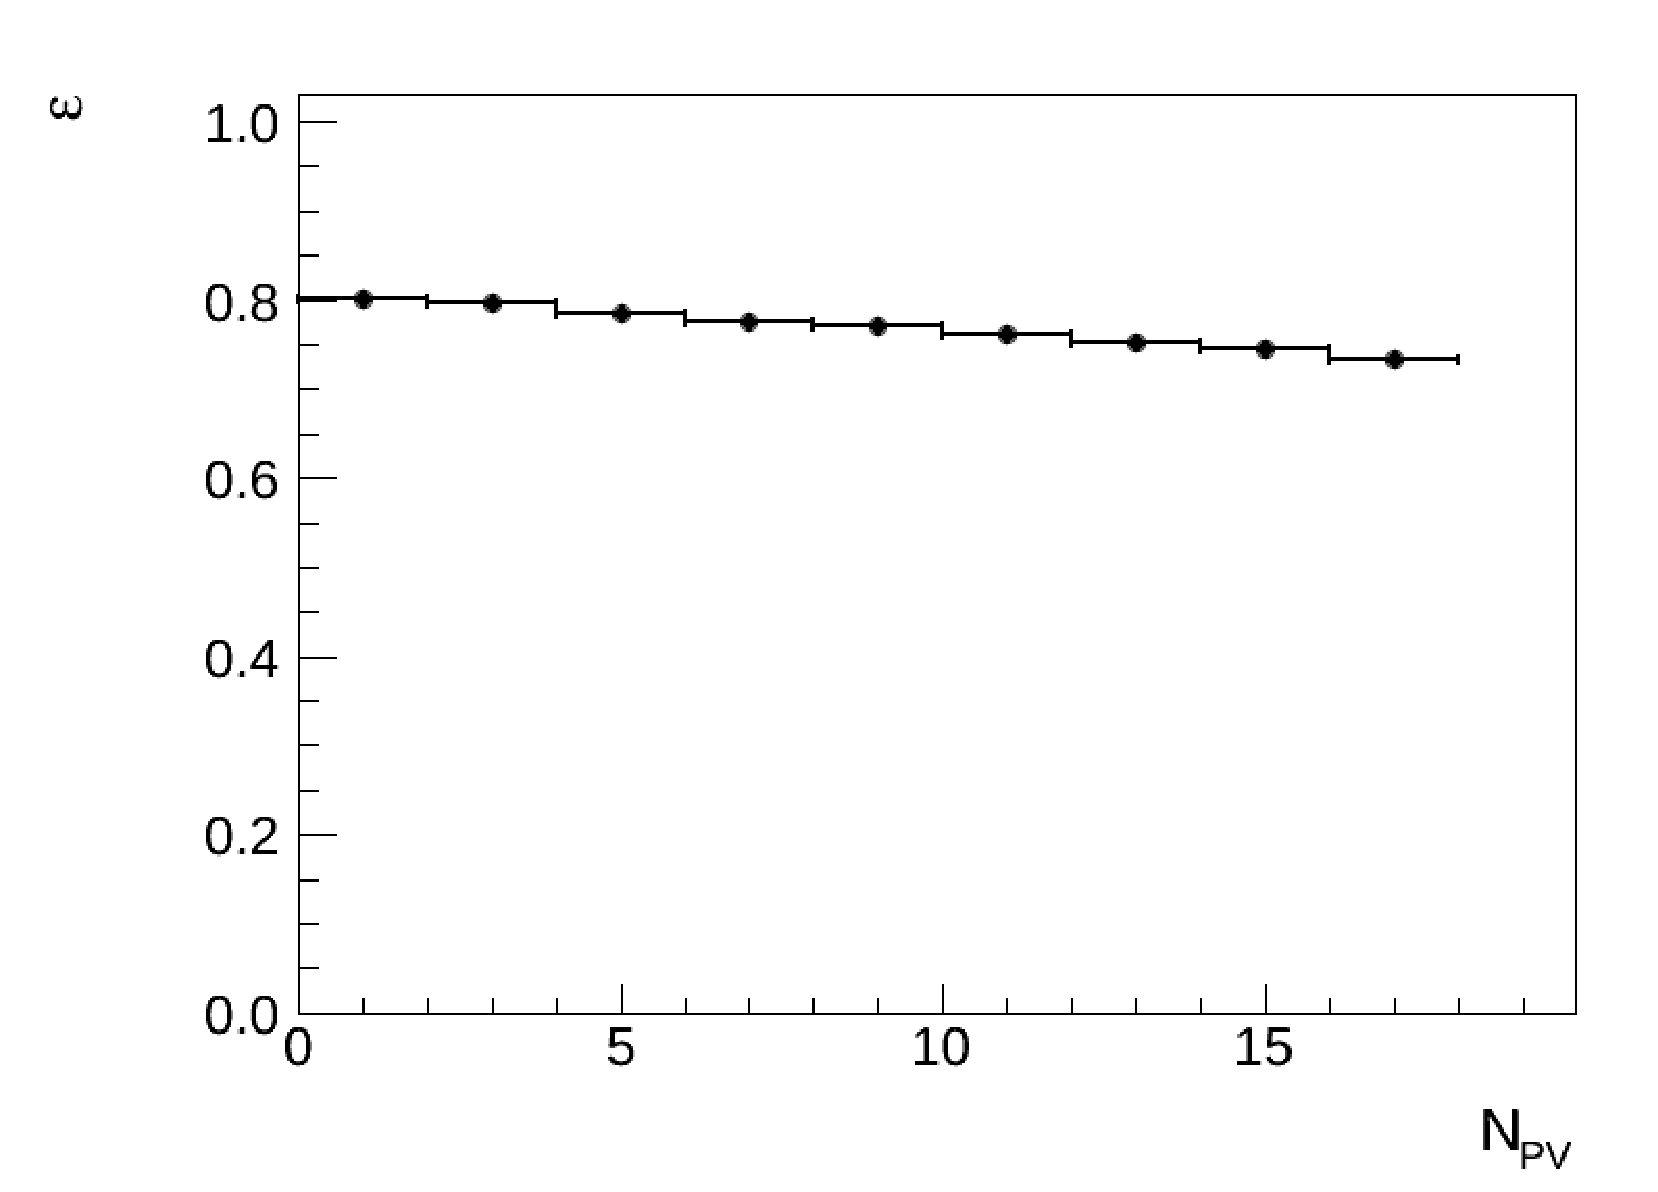
\includegraphics[width=0.45\textwidth]{figures/ElectronEff_HighPt_VsNVtx.pdf}}
\subfigure[Pileup energy density ($\rho$)]{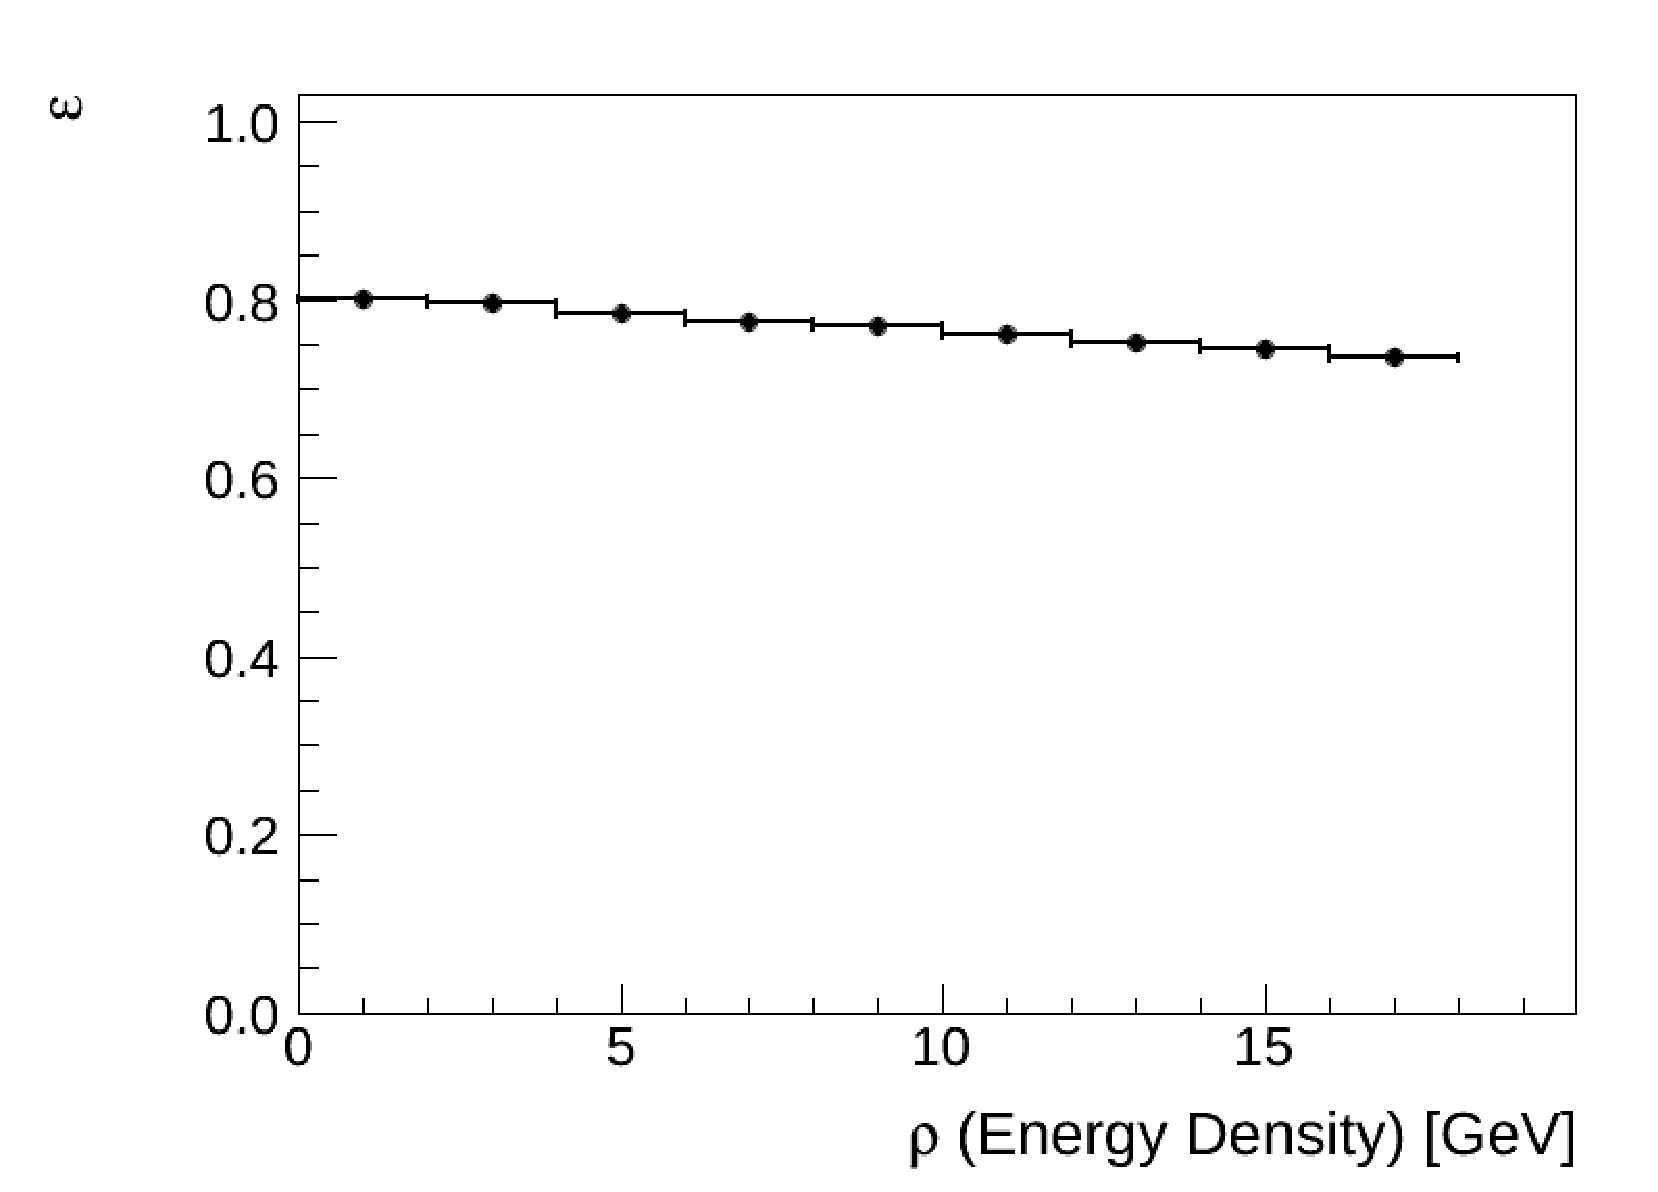
\includegraphics[width=0.45\textwidth]{figures/ElectronEff_HighPt_VsRho.pdf}}
\caption{Electron selection efficiency as a function of the number of reconstructed primary vertices
and the pileup energy density for electrons with $p_{T}$ greater than 20\GeV.}
\label{fig:ele_selectionEfficiency_HighPt_VsPileup}
\end{center}
\end{figure}



